\chapter{Landscape-level control \rom{1}: modelling ash dieback}

% paper title: Large-scale control based on regional containment
% there is a surprising lack of, simplified, ash dieback models in the literature...\ciations... <-- double, triple and quadruple check!
% without host demography 
% landscape level control strategy

Previously in Chapter \ref{ch5:dispersal-model}, we considered a generic $SIR$ dispersal model that spread via wind. Constructing the dispersal model resolved the major problem witnessed in Chapter \ref{fig:ch4_uk_spread}, namely, the failure of the SLM to spread on a realistic host density. However, the findings of Chapter \ref{ch5:dispersal-model} lacked biological specificity and thus, came short of aiding plant health. The present chapter aims to address this by constructing a landscape-level control strategy on a simplified model of ash dieback ADB. The control strategy is largely generic, and could in principle be adapted for any wind-borne tree disease.

There has been a great deal of work carried out into the nature of control in plant and tree-based epidemics\footnote{See section \ref{chapter2:plant-ecologoy} for a review on the control in plant-based epidemics.}. In particular, the spatial structure of plant-hosts is an essential factor when considering how to manage an outbreak \cite{spatial-control-optimisation, control-heterogeneous-landscapes}. The accepted paradigm of control typically considers infected tree removals over a relatively small spatial scale, near infected hosts \cite{WEBIDEMICS}, or more broadly, ahead of the wavefront \cite{large-scale-control}. However, landscape-level epidemic control, based solely on the structure of large-scale spatial distribution of hosts incorporating topography, has yet to be explored in-depth.\\

As such, in this chapter, we will examine how host-heterogeneity, under the influence of a wind-dispersed pathogen, can give rise to natural pinch-points and fault lines in the spatial distribution of hosts. Population pinch points may give rise to a bottleneck in the epidemic spread, which in principle, may be exploited with targeted tree felling to fragment the host population with minimised effort. In essence, a strategy of 'regional containment', targeting the local wind-based pathogen dispersal mechanism, is formulated and scaled up over large spatial scales. Similar concepts for crop and livestock diseases have been outlined \cite{PAPAIX201435, GILIOLI20131, Gilligan-disease-management}, however, to our knowledge, this has not been generalised to tree population distributions over large spatial scales.

A simplified $SEIR$-type model of ash dieback is developed to demonstrate this control strategy, alongside an appropriate definition of the reproductive ratio\textemdash denoted by $R_0$. The value of $R_0$ is projected onto the map of ash tree canopy cover in GB, as given by \cite{hill.data}. From the $R_0$ maps we construct, a simple notion of epidemiological connectivity can be defined and visualised through a susceptible '$R_0$-cluster' over the population of GB ash trees. This leads us to develop a heuristically-based fragmentation algorithm. As we define it, fragmentation considers which locations in the population, if artificially taken below $R_0 = 1$ through felling, would disrupt epidemiological connectivity\textemdash, thus leading to containment. Epidemic containment in the largest $R_0$-cluster is then analysed and shown to be most applicable over a specific range of infectivity parameters.

It is widely accepted that ADB will wipe out the vast majority of ash in Great Britain over the next few decades \cite{ash-dieback-costs}. Therefore, large-scale control efforts aim to slow the spread, in contrast, to complete containment. % Find references of current efforts/guidelines 
A slower rate of spread benefits ash populations allowing them to recover alongside artificial replanting.% reference 
Although the strategy of control presented in this chapter is demonstrated on a simplifed model of ADB, the results are generic and could be applied to any wind-dispersed pathogen.
The pathosystem ADB presents an interesting and relevant case study of an emerging epidemic whose reproductive mode is both seasonal and subject to LDD. The]refore, a model of ADB brings together the several key elements of chapter \ref{ch5:dispersal-model}, measuring $R_0$ over different temporal and spatial scales. 

The challenge of controlling ADB primarily reflects the challenge of containing a pathogen that spreads via long-distance dispersal (LDD). As such, developing a landscape-level control strategy when there is LDD (and epidemic uncertainty) present several obstacles that must be acknowledged beforehand. Firstly, the complexity of modelling ADB is a thesis in and of itself, few parameters are known, spatial and genetic variations are significant \cite{stocks2017first, mckinney2014ash} and a dependency on the landscape \cite{doi:10.1111/1365-2745.13383}. Moreover, HP can infect ash through diverse mechanisms such as water-course and contaminated soil and LDD means that new and distant foci can emerge over large distances without the need for nearby ash\textemdash for a more detailed review of ADB, including the challenges of control and biology, see chapter \ref{chapter2:litrevieiw}.

multi-scale approaches have been outlined \cite{hart2020theoretical}
multi-seasonal frameworks comprise a common theme in the spread of crop-based epidemics see  x, y, and typically involve soil-borne nematodes-based outbreaks \cite{tankam2020modelling} <- see references inside.
ash dieback has a strong morality rate \cite{stocks2017first}

\section{Constructing an $SEIR$ model}

\subsection{On the biology of ash dieback}

The primary infection mechanism occurs when the fungal spores of \textit{H.pseudoalbidus} (HP) are wind-dispersed in the summer and land on the leaves of susceptible ash. Once the pathogen colonises a leaf, it spreads to the xylem and then throughout the whole tree. % references on mechanism
An infected tree will then shed its leaves in the autumn. Fungal fruiting bodies then grow on dead leaf litter until summertime; at that point, spores produced by the fruiting body are wind-dispersed and continue the cycle by producing new secondary infections.% expand on the fruiting body spore production.

Specific to ADB, there are two stages of dispersal: the causal agent HP is dispersed on infected leaves during the yearly shed of ash, secondly, wind dispersal of fungal spores. Fortunately, the aggregate behaviour of two-stage dispersal is captured by sampling the amount of fungal spores with distance from a nearby source of infected ash \cite{grosdidier2018tracking}\textemdash discussed more below. 
Be that as it may, an infected tree is treated as the dispersal site in the model, although the realistic description is not so simple.

The life cycle can be understood to have two phases of growth, sexual and asexual. % reference
The asexual phase occurs when the pathogen infects and amplifies through the host \textcolor{red}{and occurs all year round}. The sexual phase of HP occurs during the summer months, from June until September when wind-dispersed spores infect new ash trees. % double check the red-highlighted

The seasonal infection cycle of ADB resembles that of crop-based disease \cite{tankam2020modelling}. Although, in the context of crop disease, removal usually coincides with harvest time. In contrast, ash infected with HP can be removed by the pathogen over a time frame spanning years. Once infected, the time ash survive depends on a plethora of factors such as age, surrounding landscape, genetic susceptibility or the particular mode of pathogen infection\footnote{For example, the pathogen can colonise the root-system \cite{schumacher2011general}, usually in severely infected ash \cite{https://doi.org/10.1111/mpp.12073}. From this point, it is only a matter of time before opportunistic fungi invade and significantly accelerate mortality \cite{enderle2013temporal}.}. In Germany, a forest stand of planted ash trees had a $73\%$ mortality rate after five years \cite{langer2015ash} (as cited in a review \cite{enderle2017ash}), while observations of ADB progression in Austria suggest a low mortality rate of $5\%$ measured over a two-year window \cite{kessler2012dieback}. Furthermore, a study conducted at different sites throughout England suggests a time-scale ranging between $3-15$ years of infected tree growth before death \cite{wylder2018evidence}.

% The mortality of infected ash infected with HP is high, recent estimates suggest around $95\%$ \cite{stocks2017first}. % check \cite{ash-dieback-costs} paper for other estimates

\subsection{Infection dynamics}
\label{sec:infection-dynamics}

\begin{table}[h]
\centering
\begin{tabular}{l l l}
\hline
\textbf{Model parameter} & \textbf{Description} & \textbf{Value(s) taken}\\
\hline
$\rho$  & Tree density & $0.00 - 0.10$ \\ 
$\beta$ & Infectivity & $0.00010 - 0.00100$ \\
$\ell_{ga}$ & Gaussian dispersal scale parameter& $196\mathrm{m}$ \\
$\ell_{pl}$ & inverse power dispersal law scale parameter& $203\mathrm{m}$ \\
$a$ & Inverse power law exponent & $3.3$ \\
$T$ & Sporulation peak & June - September \\
$t$ & Time-step & $1\ \mathrm{day}$\\
$R_0$ & Mean reproduction number & $0-20$ \\
$\mathcal{L}$ & Lattice dimension & $1000\times1000$ \\
$\mathcal{A}$ & Domain area & $5\mathrm{km}\times5\mathrm{km}$ \\
$\gamma$ & Lattice constant & $5\mathrm{m}$ \\
$\mu$ & Peak leaf-shedding of ash & November \\
$\sigma$ & Leaf-shedding standard deviations & 2 weeks \\
$\lambda$ & Mean exponentially-distributed infectious life-time  & $5\ \mathrm{years}$ \\
\hline
\end{tabular}
\caption{Parameters used in the $SEIR$ model of ash dieback. The dispersal parameters are taken from \cite{grosdidier2018tracking} and the typical tree densities of ash are informed from by \cite{hill.data}.}
\label{tab:SEIR-model}
\end{table}

As before, the hosts' distribution, in this case ash, is initialised by a Bernoulli trial with probability $\rho$ according to a binomial distribution\textemdash thus giving rise to a flat and randomly distributed landscape of trees. The probability $\rho$ defines the host density inside a square domain of size $\mathcal{L}$. Each lattice point is chosen to represent a $5\mathrm{m}\times5\mathrm{m}$ patch of land that approximates the canopy cover of an ash tree, this resolution yields an upper bound of $400$ ash trees per hectare of canopy cover \cite{ash-tree2, ash-tree1}.

However, this time, we include an extra latently infected (or exposed) compartment, denoted by $E$, into the model. Thus, a tree can be in one of four compartments and transition through $S\rightarrow E \rightarrow I \rightarrow R$, without the possibility of recovery. Figure \ref{fig:SEIR-transitions} shows a typical scenario; an infected ash tree in the $n^{th}$ cycle, or equivalently $n$ years after the initial outbreak, may infect ash in the $S$ compartment. Newly infected ash will transition into the $n^{th}$ $E$ compartment, denoted by $E_n$, and become infectious in the following year $I_{n+1}$. 

In the $E$ compartment, trees are latently infected i.e. infected but not infectious. % REFERENCE
The compartments $(E_1, E_n,..,E_n)$ do not represent different biological states. The index $n$ is included for convenience to highlight the fact that in this model, it takes latently infected ash takes approximately one year to start produce new secondary infections during the $(n+1)^{th}$ sporulation peak.

\begin{figure}
    \centering
    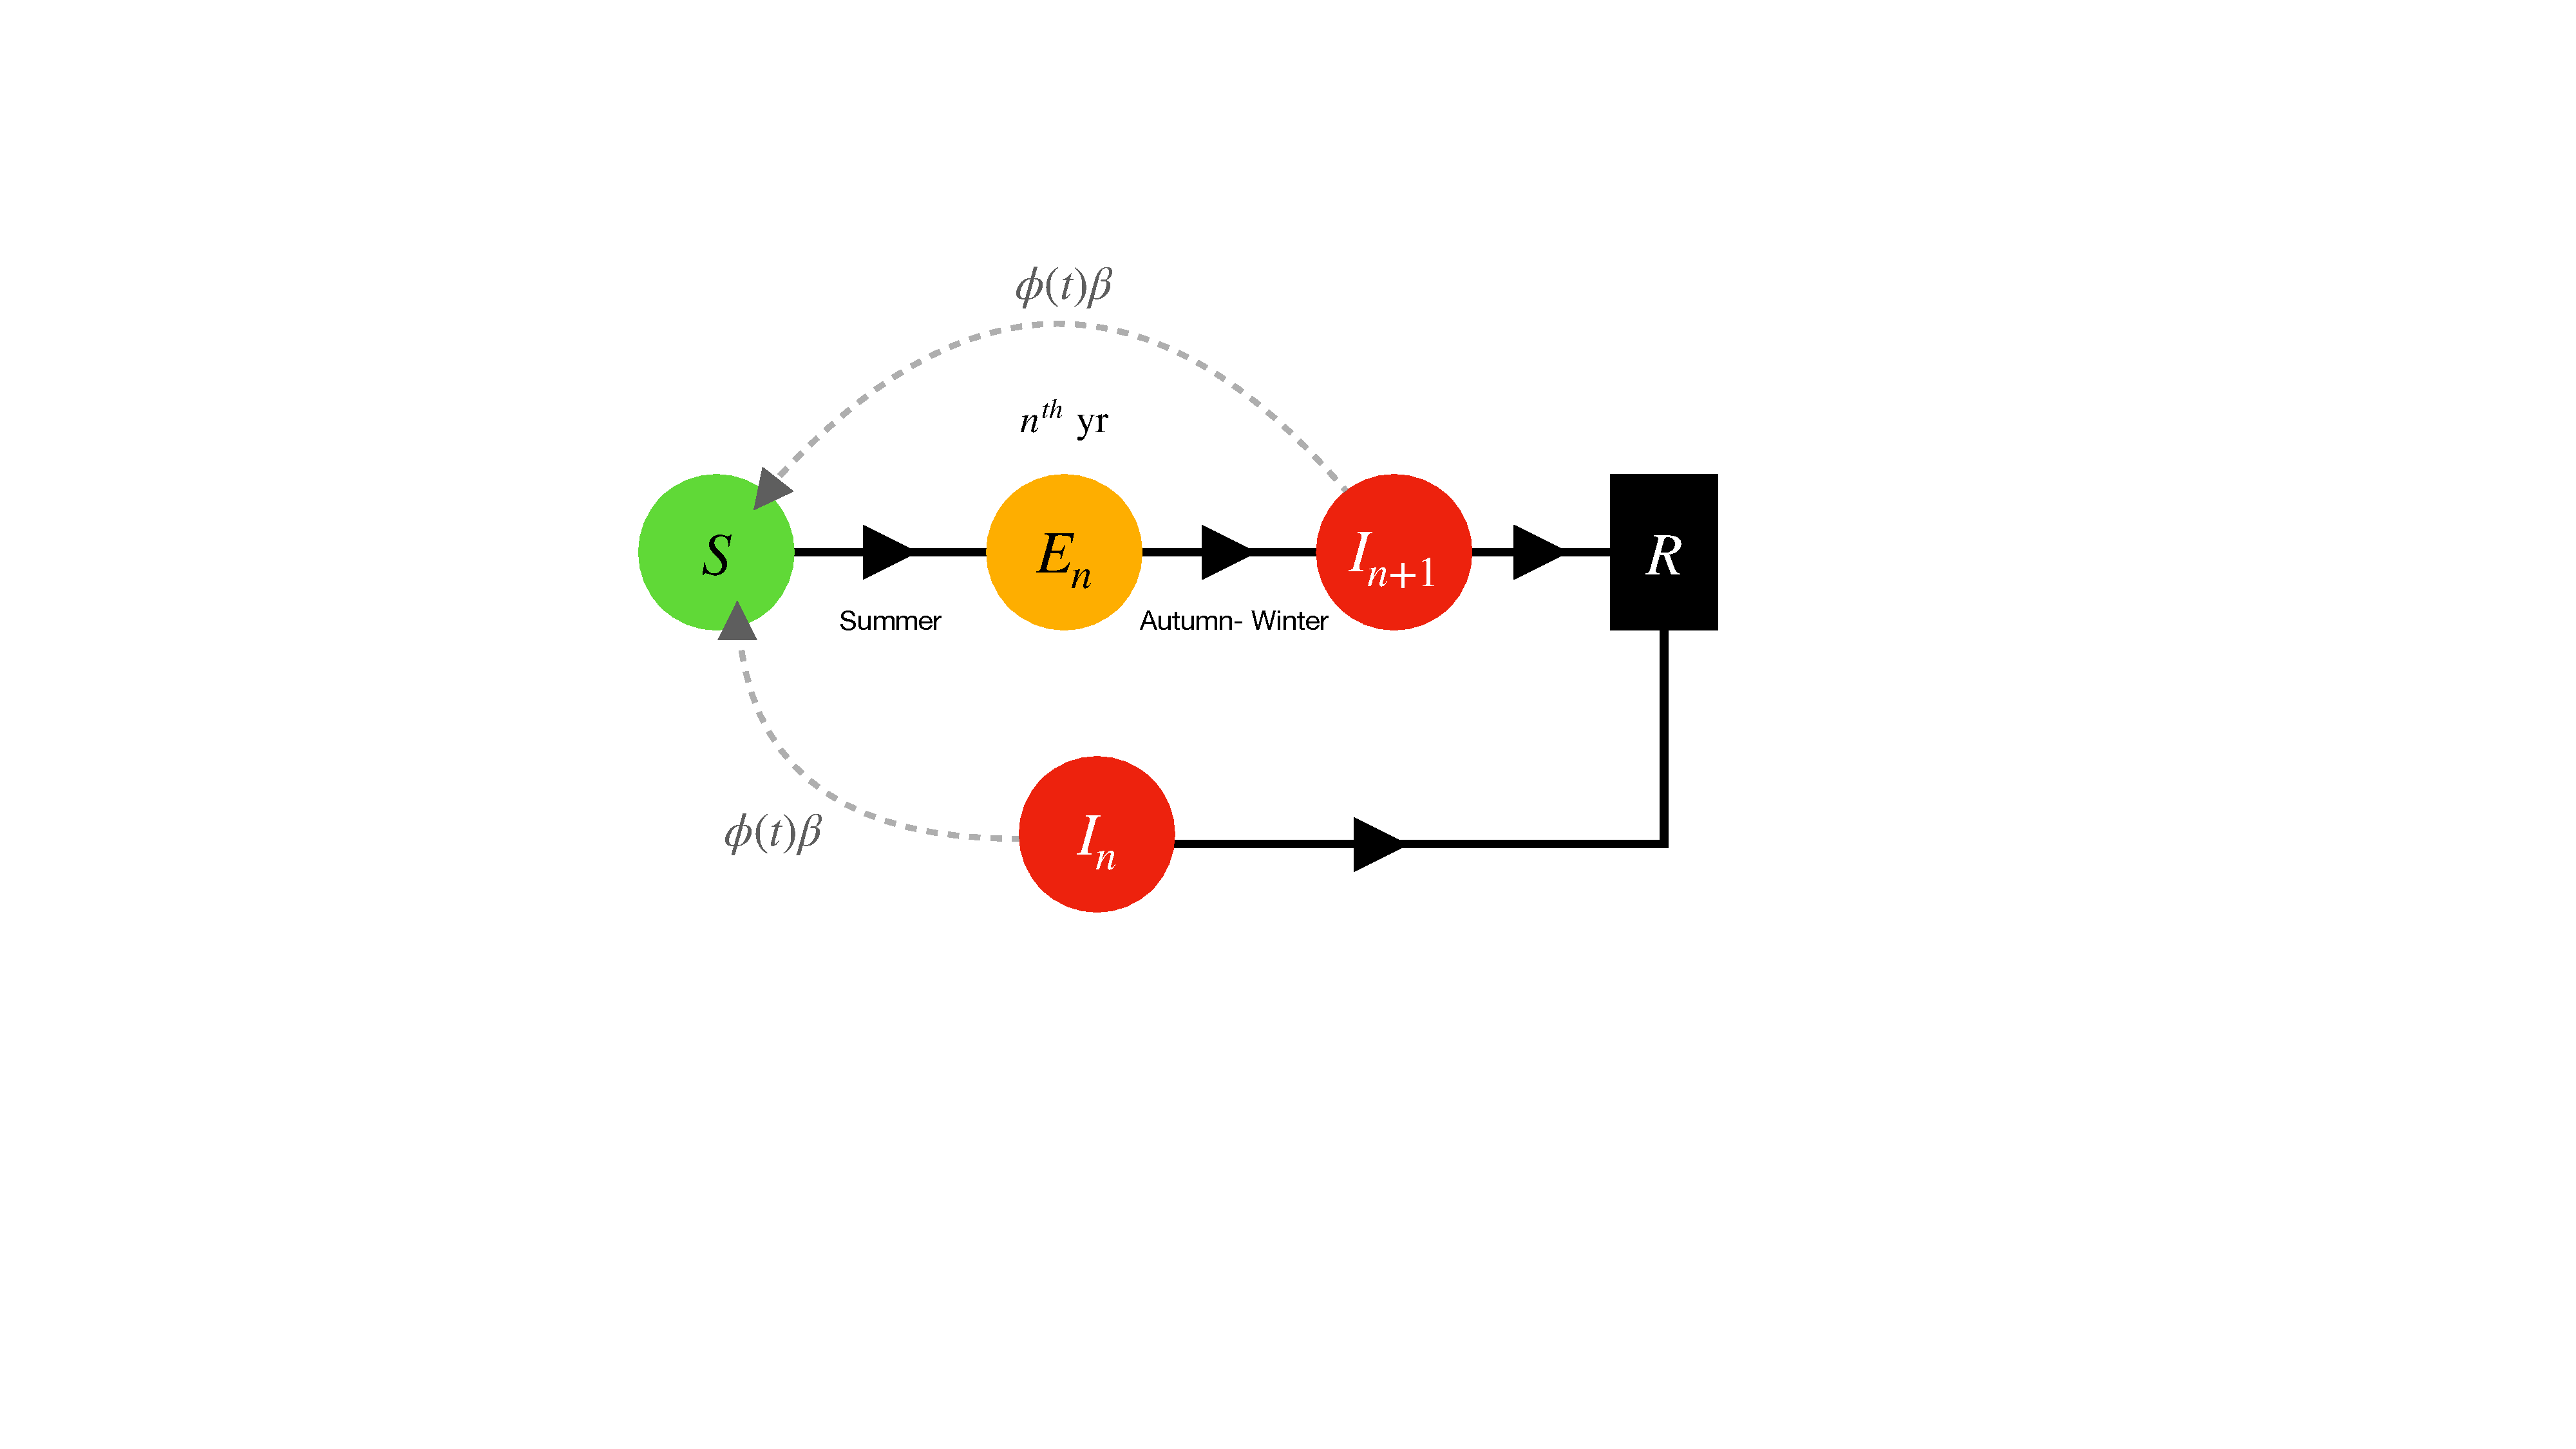
\includegraphics[scale=0.30]{chapter6/figures/fig1-seir-transitions.pdf}
    \caption{The seasonal $SEIR$ model of AD. In year $n$ of an outbreak, an infectious tree may cause a transition $S\rightarrow E_n$ during summer, depicted by the bottom dashed grey arrow. A tree that becomes latently infected in year $n$ will lead to an infectious tree in year $n+1$. Eventually, all infected ash are removed without the possibility of recovery.}
    \label{fig:SEIR-transitions}
\end{figure}

As defined here, a latently infected ash tree in $E_n$ transitions into the infectious compartment $I_{n+1}$ during seasonal leaf shedding between Autumn and Winter. A Gaussian distribution centred in November with a two-week standard deviation represents this in the model. This particular choice of distribution and standard deviation, although intuitive, is ultimately ill-informed. However, because infected ash do not produce any secondary infections until the following summer, we can afford some degree of flexibility modelling the exact timing of transitions between $E_{n}\rightarrow I_{n+1}$ during Autumn and Winter; provided exposed ash transition into the infected compartment before sporulation, the epidemic spread will remain the same.

Once in the infectious compartment, an infected ash tree will not give rise to any secondary infections until summer when fruiting bodies on dead ash leaf litter produce ascospores. Thus, infectivity in the model should be time-dependent, this is captured by a 'sporulation' function $\phi(t)$. Sporulation functions have been investigated in the context of time-varying infectivities \cite{time-varying-infectivity}. In the case of ADB, the function $\phi(t)$ is used to mirror the life cycle of ADB where new secondary infections only arise during the summertime sporulation \cite{https://doi.org/10.1111/mpp.12073}. That is, non-zero from June until September, and zero otherwise\footnote{Variations in ADB sporulation have been noted between European countries \cite{https://doi.org/10.1111/mpp.12073}, along with the potential for early-onset sporulation in the face of favourable environmental conditions. Although, the most generally agreed upon sporulation period is thought to be from June to September.}.

To model dispersal, a thin-tailed Gaussian was considered alongside a fat-tailed inverse power law distribution\textemdash see table \ref{tab:SEIR-model}. A probability of transition $S_x \rightarrow E_x$ for Gaussian and inverse power law respectively, can be seen to follow:
\begin{equation}
    Pr(S_{x} \rightarrow E_{x} ;\ I_{x^{\prime}} ) = \beta  \phi(T) \exp\Big[\frac{-r^2}{2\ell^2_{ga}}\Big] 
\end{equation}
\begin{equation}
    Pr(S_{x} \rightarrow E_{x} ;\ I_{x^{\prime}} ) = \beta \phi(T) (1 - r/\ell_{pl})^{-a}
\end{equation}
where $\phi(t)$ is a time-dependant function reflecting the seasonal life-cycle of ADB and $r$ is the distance between $S_x$ and $I_{x^\prime}$. Two sporulation functions are considered, the precise functional forms are discussed below in section \ref{ch6:sporulation}. 

The inclusion of an exposed category, together with a sporulation function, constrain the dynamics of ADB whereby: A) infected ash may be latently infected and display symptoms but crucially not disperse any infectious material B) ash may shed infected leaves in Autumn/winter, and thereby disperse infected material, but not lead to any secondary infections until the following summer when ascospores are produced.

The last transition to consider is from infected to removed $I_{n}\rightarrow R$. Given a $95\%$ mortality rate, ADB can be regarded as lethal. % REFERENCE
Therefore, once an ash tree becomes infected, an eventual transition to the $R$ compartment is assumed with certainty\footnote{Interestingly, certain edge-cases can contradict this assumption. 
For example, a sufficiently large quantity of inoculum deposited on ash leaves can result in leaf shed before the infection has the chance to spread throughout the tree \cite{https://doi.org/10.1111/mpp.12073}.}. 
The precise probability distribution describing $I_{n}\rightarrow R$ is, to my knowledge, non-existent in the literature. 

As a first approximation, infected ash were chosen to have exponentially distributed life-times with a mean of five years, see table \ref{tab:SEIR-model}. 
This choice was informed by experimental observations of ash mortality after years of infection. In particular, reports of $5\%$ mortality after two years of infection \cite{kessler2012dieback}, $75\%$ mortality within five years \cite{langer2015ash} and no observations of infected ash surviving beyond $15$ years \cite{wylder2018evidence} provide some guidance towards an approximate time-scale.

However, as discussed in detail later, the main results of this chapter depend on time-scales below the mean infection life-time. So once again, there is some degree of flexibility in the precise time-scale of $I_{n}\rightarrow R$.
\textcolor{red}{Re-fame and discuss interpretation of time-scale and ash age...}


% subdividing compartments in this manner could also provide an easier implementation to hosts which become more infectious, through a greater production of spores, as the infectious cycle continues not to mention particular periods of environmental unsuitability.
% 
 
\subsection{Dispersal parameterisation}

\begin{figure}
    \centering
    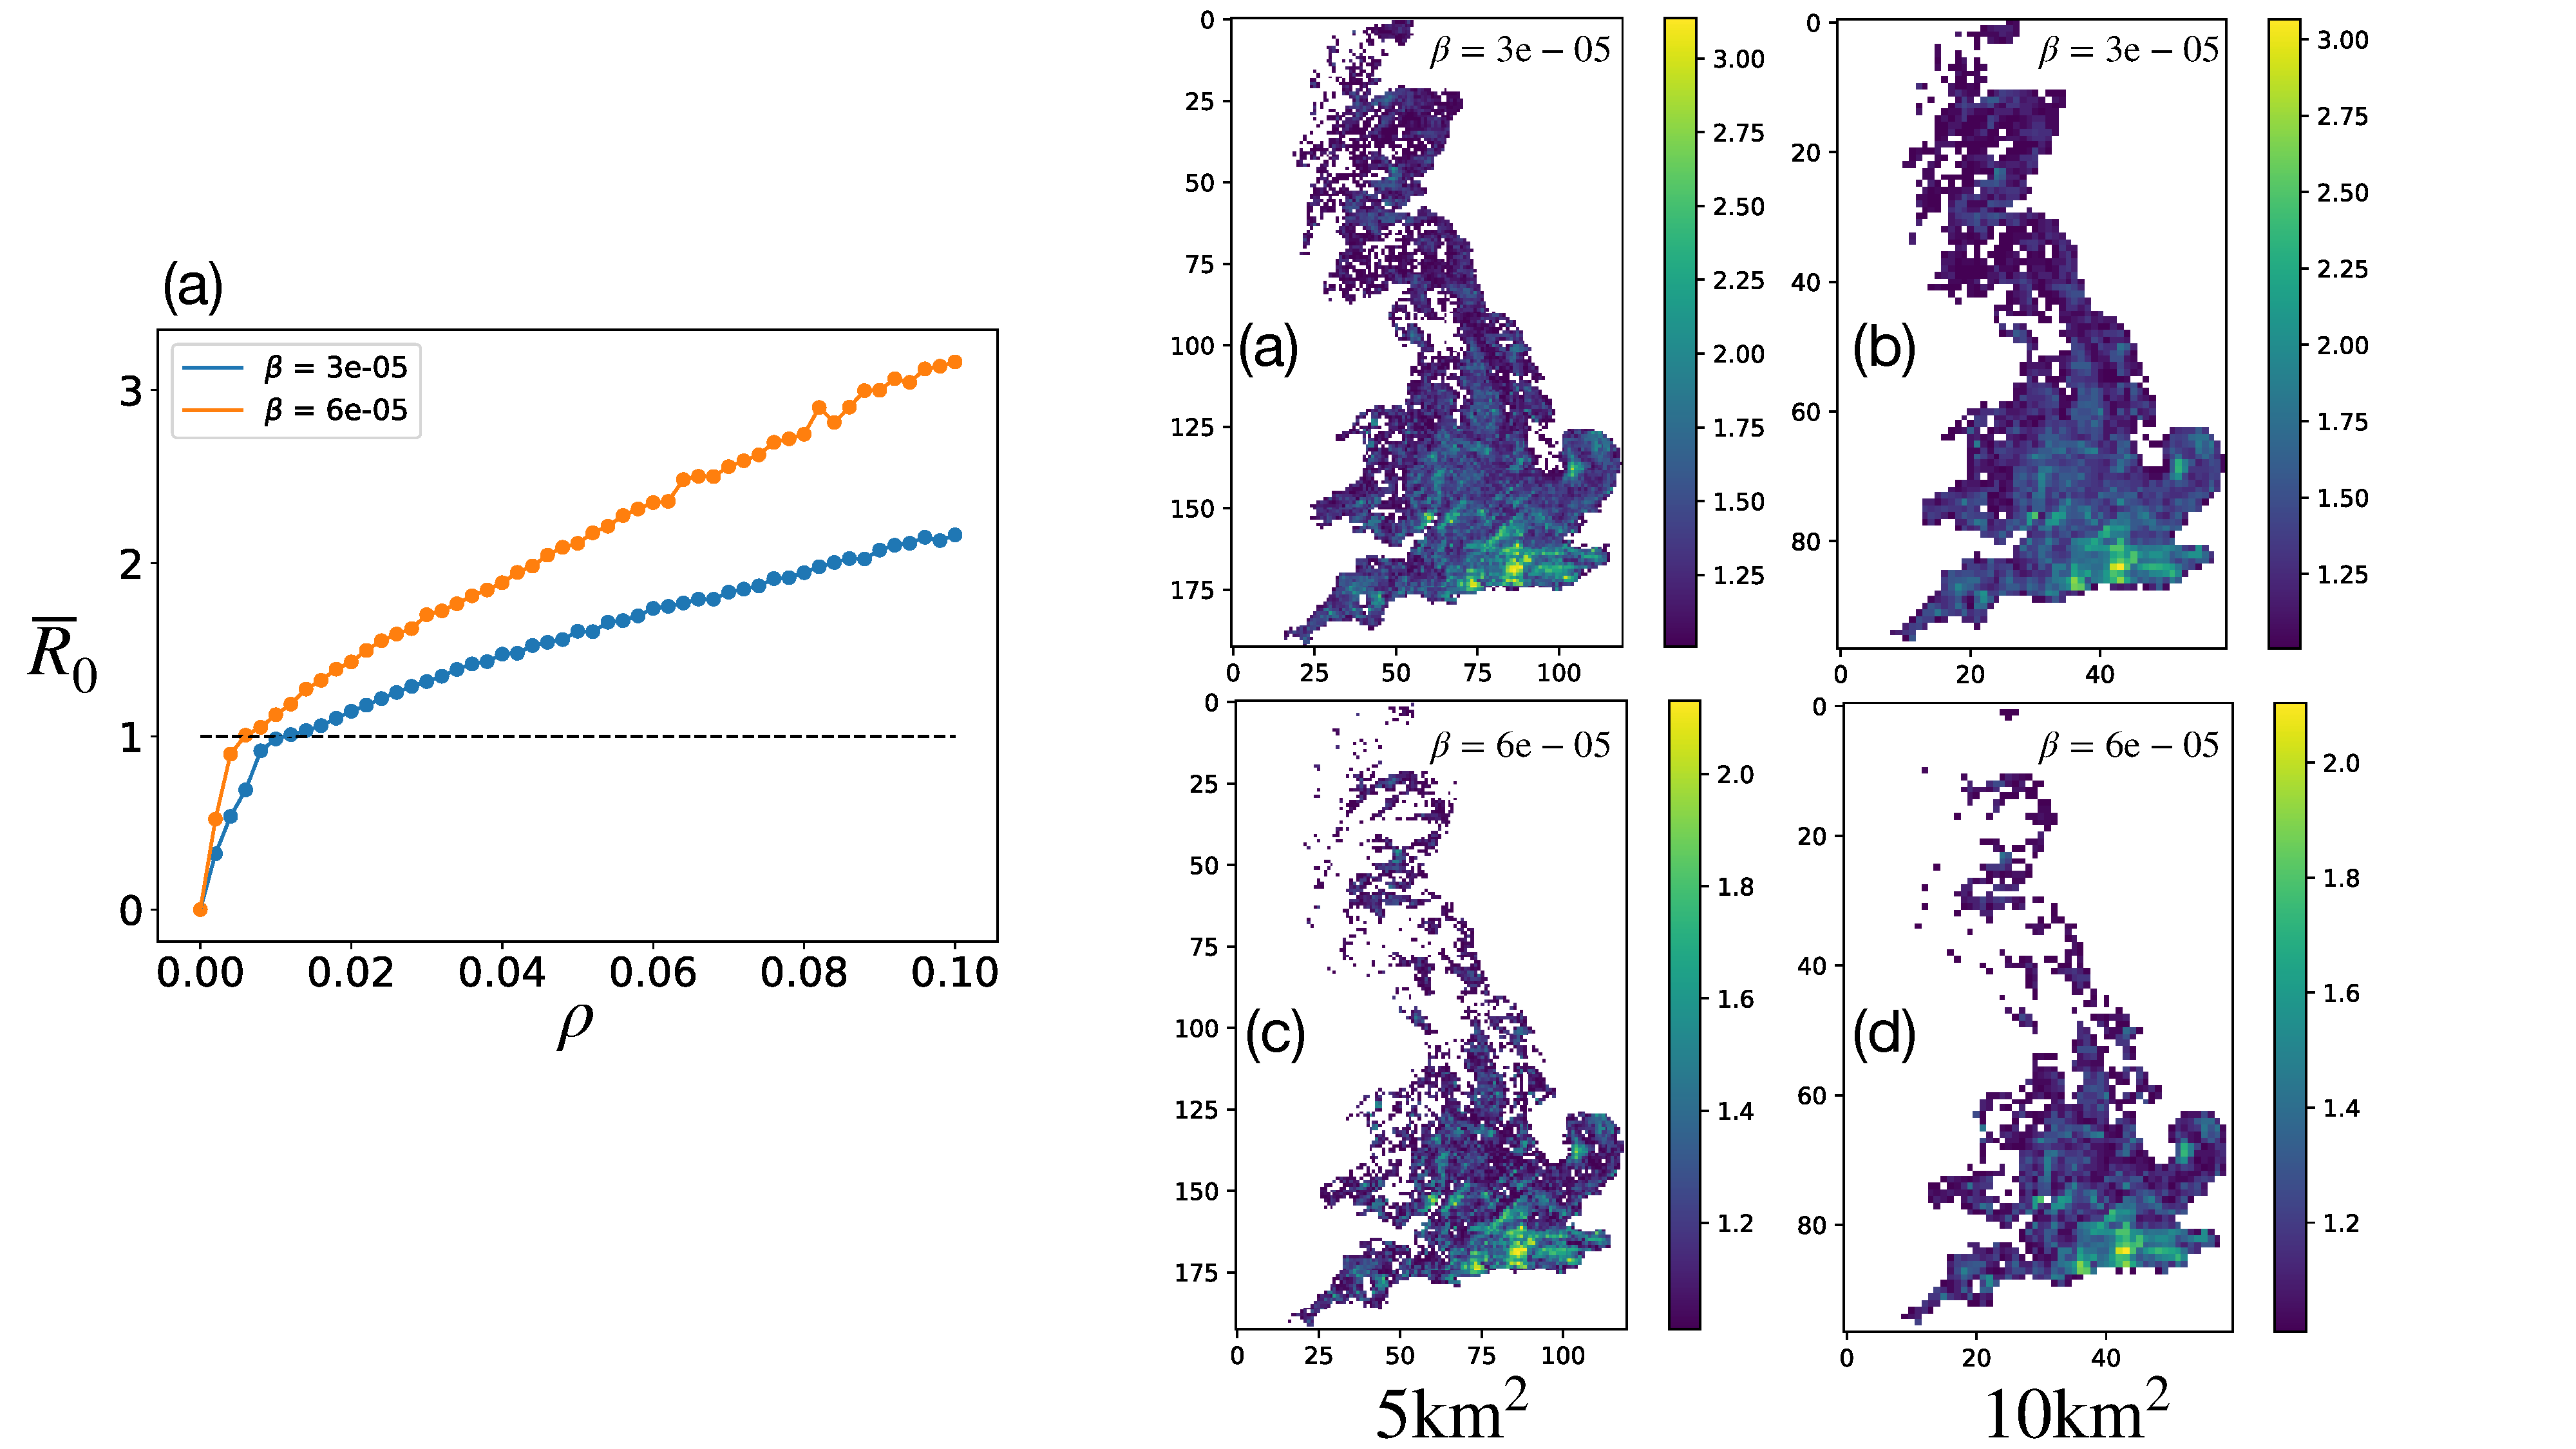
\includegraphics[scale=0.25]{chapter6/figures/fig2.pdf}
    \caption{Dispersal gradients at the local spatial scale, parameters are informed by the work of \cite{grosdidier2018tracking}. The authors provide estimates for Gaussian and inverse power law kernels: $\ell_{ga} = 195\mathrm{m}$ and ($\ell_{pl} = 205\mathrm{m}$, $a=3.3$) respectively, where $a$ represents the inverse power law exponent.}
    \label{fig:dispersal-parameterisation}
\end{figure}

Dispersal was informed by data collected in France by \cite{grosdidier2018tracking}. The field study conducted by \cite{grosdidier2018tracking} provide estimates for dispersal parameters by fitting data against a Gaussian and inverse power law kernels. Notably, the authors studied dispersal at two different spatial scales, local and regional, \textcolor{red}{on the order of $1\mathrm{km}$, to $10-100 \mathrm{km}$ respectively}. For a review on the importance of scale, see chapter \ref{chapter2:litreview}. 

The experimental data analysed by \cite{grosdidier2018tracking} tracked ADB spores about known sources of infection. Although data on spore depositions does not necessarily correspond to a new infection, it sheds essential light on the spatial scale of ADB dispersal. Given that the spatial scale in the $SEIR$ model is small, at a  resolution of $5\mathrm{m} \times 5\mathrm{m}$, a decision was made to parameterise dispersal with the local-level dispersal values given by \cite{grosdidier2018tracking}. See table \ref{tab:SEIR-model} an Fig\ref{fig:dispersal-parameterisation}. 

The decision to use ADB scale parameters given by \cite{grosdidier2018tracking} suppose that the spread of ADB in Great Britain is comparative to the spread of ADB in France. Nonetheless, there is a noticeable difference in the French climate, landscape and, importantly, wind patterns. % references
Notwithstanding these differences, it stands to reason that dispersal parameters, if measured over a smaller, local spatial scale, would be less pronounced. 

Lastly, the regional-scale dispersal analysed by \cite{grosdidier2018tracking}, measured over spatial scales of $10$-$100\ \mathrm{km}$, is thought to contain artefacts of LDD by human-mediated transport. The regional spread of ADB though LDD is, therefore, beyond the scope of the present chapter\textemdash a discussion of LDD will conclude this chapter and lead us to chapter into chapter \ref{ch7:pde}.

% Q: what is the relationship between the mortality ratio (or final fraction of infected hosts) ? 
% If R0 was considered over a larger time-scale, host-regrowth would need to be integrated into the model
% Furthermore, measuring R0 over a larger time-scale could over, or underestimate, the degree to which a response would need to be undertaken in the response time-window. 
% a basic reproduction number $R_0$ is defined for the first life-cycle of the pathogen.
% Moreover, data over a relatively short time scale is typically all that is available when making decisions about control, not to mention the added complexity of incorporating host-regrowth–which becomes an important factor over longer time scales–and so, the constraint of computing R0 over longer time scales is relaxed. 
%  We develop the simplest implementation possible, namely, where R_0 is measured over one pathogen life-cycle, and the course of infection for each host follows the same process with perfect fidelity. This lies in stark contrast to a realistic scenario whereby different hosts show considerable differences.

% \begin{itemize}
%     \item see for a review on how R0 is calculated \cite{perspectives-on-r0}, we use method x in order to estimate and inform R0
%     \item $R_0$ is a complex function which changes in time, to this end, the next generation operator is used to derive a value for $R_0$ \cite{doi:10.1098/rsif.2009.0386}. In order to inform the value of $R_0$ we do xy and
%     \item Although it is hard to enforce a true $R_0$ value, the most important feature introduced from the definition is a threshold from which we can see if a local invasion is likely to take place.
%     \item Since the number of susceptible hosts is fixed, without replacement, the number of susceptible hosts will continually decrease in time in the case of an epidemic. Given the strong spatial component in the model we expect that measuring $R_0$ as-per this definition will give an under-estimate for later times when few susceptible trees remain. Likewise, for earlier times when susceptible neighbours are plentiful $R_0$ will yield an upper estimate for the pathogen. In order to characterise the pathogen in this model, we take the upper bound defined between the $1^{st}-2^{nd}$ generations. This simplification represents a worst-case scenario and the mean value of $R_0$ would be lower for later times when there are less trees available to infect. But most importantly, the threshold of transmission $R_0>1$ is reliable captured \textit{during the initial stage of infection}.
%     \item $R_0$ can be fully characterised by a growth rate \cite{R0-construct}. That is, the growth factor per generation.
% \end{itemize}

\section{Seasonal $SEIR$ model behaviour}

Previously in section \ref{sec:infection-dynamics} the details of sporulation were omitted. For robustness, two sporulation functions are considered, a step function defined by equation \ref{eq:step-function} and a normal distribution located at the midpoint between June and September. For now, the simplest form of sporulation is adopted: % DISCUSS PLANK SPORULATION...
\begin{equation}
\label{eq:step-function}
\phi_1(t) = 
\begin{array}{cc}
  \{ & 
    \begin{array}{cc}
      1 & t\in [\mathrm{June},\ \mathrm{September}] \\
      0 &  \mathrm{elsewhere}
    \end{array}
\end{array}
\end{equation}

The $SEIR$ model behaviour is shown in Figure \ref{fig:SEIR-spread} for the inverse power law dispersal model over the average density of ash in Great Britain.
The Gaussian-based dispersal model displays the same seasonal behaviour, as demonstrated in appendix \ref{section:ga-SEIR-variant}. For each year after outbreak, a rise in the number of latently infected ash in $E$ can be seen during summertime sporulation, June-September, followed by a rise in the number of infectious ash in the Autumn-Winter. 

The spatial progression of ADB in the $SEIR$ model is shown in Figures \ref{fig:SEIR-spread}(a-c) over one year. The simulation begins in Figure \ref{fig:SEIR-spread}(a) with an initial condition of $25$ infected ash distributed throughout the host landscape during March. At this point in the year, fungal fruiting bodies on infected leaf litter will be preparing to release ascospores.
During the sporulation season, secondary infections are produced, and latently infected ash spread throughout the domain, depicted by the orange dots in Figure \ref{fig:SEIR-spread}(b). After the sporulation season ends in September, latently infected ash begin to transition into the $I$ compartment, reflected by the increased number of red dots in Figure \ref{fig:SEIR-spread}(c). The cycle will continue when the next cohort of secondary infections are produced in the following summer when the sporulation function next becomes non-zero.

The number of ash in the $SEIR$ compartments (on logarithmic axes) is shown in Figure \ref{fig:SEIR-spread} for three infectivity parameters in a $2\mathrm{km}\times2\mathrm{km}$ domain. Figure \ref{fig:SEIR-spread} shows three scenarios over $10$ years with infectivity parameters $\beta \in [2.5\times 10 ^{-4}, 1.5\times 10 ^{-4}, 1.5\times 10 ^{-5}]$, above, around and below the epidemic threshold, (d-f) respectively. In Figure \ref{fig:SEIR-spread}(d), $\beta$ is above the epidemic threshold and the number of ash in $S$ decline rapidly, shown by the blue line. During seasonal sporulation, large spikes in the number of latently infected ash can be seen in orange. Latently infected ash quickly transition into $I$ during Autumn and winter, as shown by the seasonal rise of $I$ in green.

\begin{landscape}
\begin{figure}
    \centering
    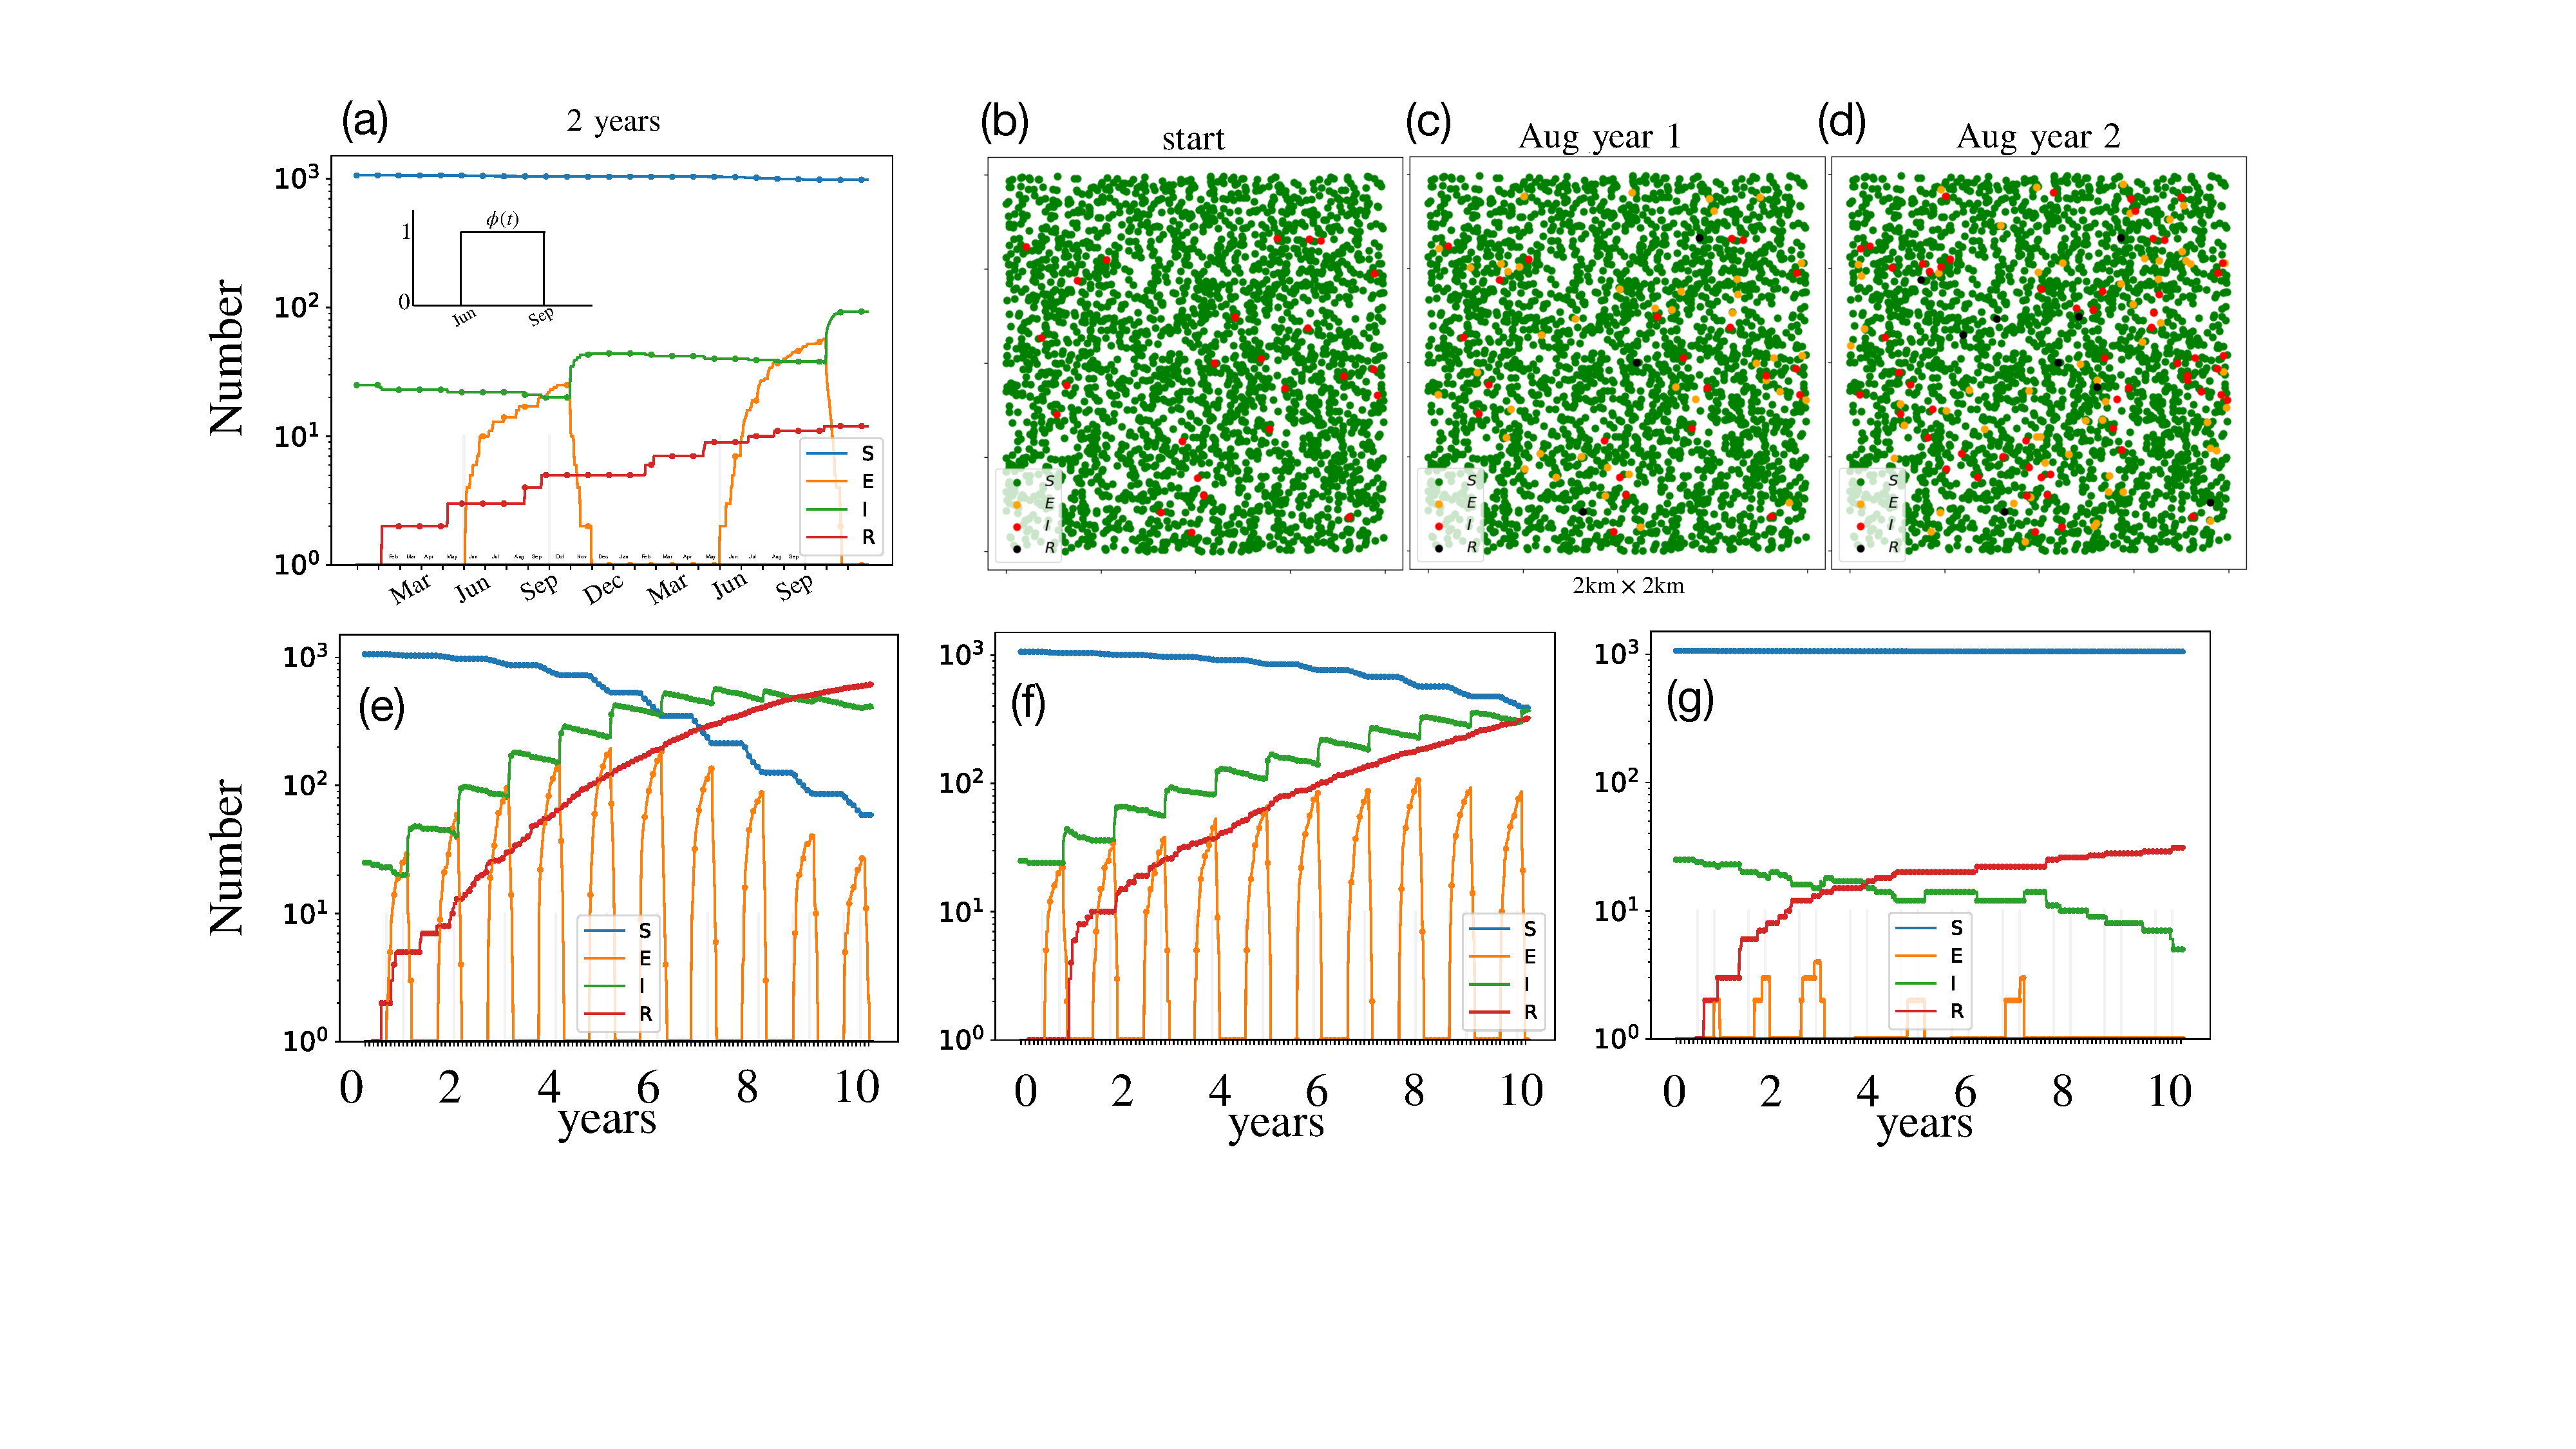
\includegraphics[scale=0.45]{chapter6/figures/fig4-seir.pdf}
     \caption{The inverse power law $SEIR$ model of ADB shown over the average ash density $\overline{\rho} = 0.017$. (a-c) The spatial progression of disease in a $2\mathrm{km} \times 2\mathrm{km}$ domain over one sporulation season beginning with $25$ infected ash distributed throughout the domain. (d-f) The number of ash in the $SEIR$ compartments are shown over ten years for infectivity parameters above, around and below the epidemic threshold respectively.}
    \label{fig:SEIR-spread}
\end{figure}
\end{landscape}

In Figure \ref{fig:SEIR-spread}(e) infectivity parameters are slightly above the epidemic threshold and the model behaviour is similar, albeit with a slower seasonal decline and rise in $S$ and $I$. For infectivity parameters below the epidemic threshold, Figure \ref{fig:SEIR-spread}(f), $S$ remains approximately constant and $I$ slowly declines. Interestingly, Figure \ref{fig:SEIR-spread}(f) persistence in model of ADB; whereby, even if the epidemic parameters are below the threshold, the fungus may survive for long periods of time. In general, persistence in plant-based pathogens is one aspect that complicates epidemic control\textemdash see chapter \ref{ch3:invasions_and_persistence} for a review of invasion and persistence in the spread of plant-based diseases

\subsection{Sporulation: time-varying infectivity}
\label{ch6:sporulation}

Time varying infectivity rates are an important concept in epidemiology, this is true for the spread of disease in both human/animal \cite{svensson2007note, liu2012infectious} and botanical populations \cite{suffert2018some, leclerc2014estimating, time-varying-infectivity, van2013plant}; this holds true for ADB. The time varying infectivity of ADB is modelled by two sporulation functions, $\phi_1(t)$ and $\phi_2(t)$, based on the work of \cite{time-varying-infectivity}. That is, a step function, and a Gaussian\footnote{Here, the Gaussian sporulation function $\phi_2(t)$ is a special case of the Gamma(k) presented in \cite{time-varying-infectivity} i.e. by taking the limits of $m$ and $n$ in the more general $SEmInR$ model.}, as shown on the insets of Figures \ref{fig:SEIR-sporulation}(a-b) respectively. 
A detailed review on the work of \cite{time-varying-infectivity} is conducted in chapter \ref{ch2:lit-rev-compartmentalised-models}.


The authors of \cite{time-varying-infectivity} demonstrated that different functions of time-varying infectivity, refereed to as sporulation curves, can be represented by an $SEmInR$ model\footnote{Note, the terms $n$ and $m$ in the $SEmInR$ model given by \cite{time-varying-infectivity} are in no way related to the subscript used in Figure \ref{fig:SEIR-transitions} to describe the seasonal component of ADB.}. The sporulation functions in \cite{time-varying-infectivity} describe how latently infected plants transition into the infectious compartment, $E\rightarrow I$ as different functions of time. 


For the seasonal $SEIR$ model of ADB a slightly different interpretation was required and the sporulation functions $\phi_1(t)$ and $\phi_2(t)$ were used control the transition $S \rightarrow E$.

For the pathosystem ADB, we have the unusual case whereby a tree can disperse infected leaf litter in autumn-winter, and thus in a sense become infectious, yet not produce any secondary infections until summer.
In the model of ADB considered here, ash are categorised as infectious when leaf shedding begins in autumn-winter, however no secondary infections will be produced until summer. 
In our $SEIR$ model of ADB, a sporulation function $\phi(t)$ is therefore suited to multiply $\beta$ and control how infectivity changes throughout the year. 
The crucial difference 

the time-dependency of fruiting bodies on infectious leaf litter releasing their spores in summer

Sporulation functions in the context of ADB are well suited to model the time-dependency of fruiting bodies on infectious leaf litter releasing their spores in summer; in the seasonal model of ADB shown in Figure \ref{fig:SEIR-transitions}, this happens when ash are already in the infectious compartment. 

Applying a time-varying sporulation function to ash already in the infectious compartment, is a simplistic way of describing 
There, it makes sense to define sporulation to capture 
and yet not produce secondary infections. In the in


% % A time-varying infectious 
% In a realist scenario, the time-dependency of infectivity during ADB sporulation is unlikely to be uniform, as suggested by Equation \ref{eq:step-function}.
% Experimental observations in France by \cite{grosdidier2018tracking} suggest that spore production reaches a maximum in July-August for example. % Show Figure ? Showing plot 
% As a rudimentary tool to explore time-varying sporulation, a second 'peaked' sporulation function would therefore be useful. 
% A normally-distributed sporulation function, $\phi_2(t)$ centered in August, mid-way between June and September, is used to parsimoniously imitate the peaked appearance of Figure 2. in \cite{grosdidier2018tracking}. 
% As far as I am aware, Gaussian sporulation has not been detailed in the literature and can therefore only serve as a comparative tool.

A typical simulation with time-varying sporulation, reaching a maximal infectivity during August, is shown in Figure \ref{fig:SEIR-sporulation}(b). Despite a different scaling of $\beta$, model behaviour looks similar. With 

\begin{figure}
    \centering
    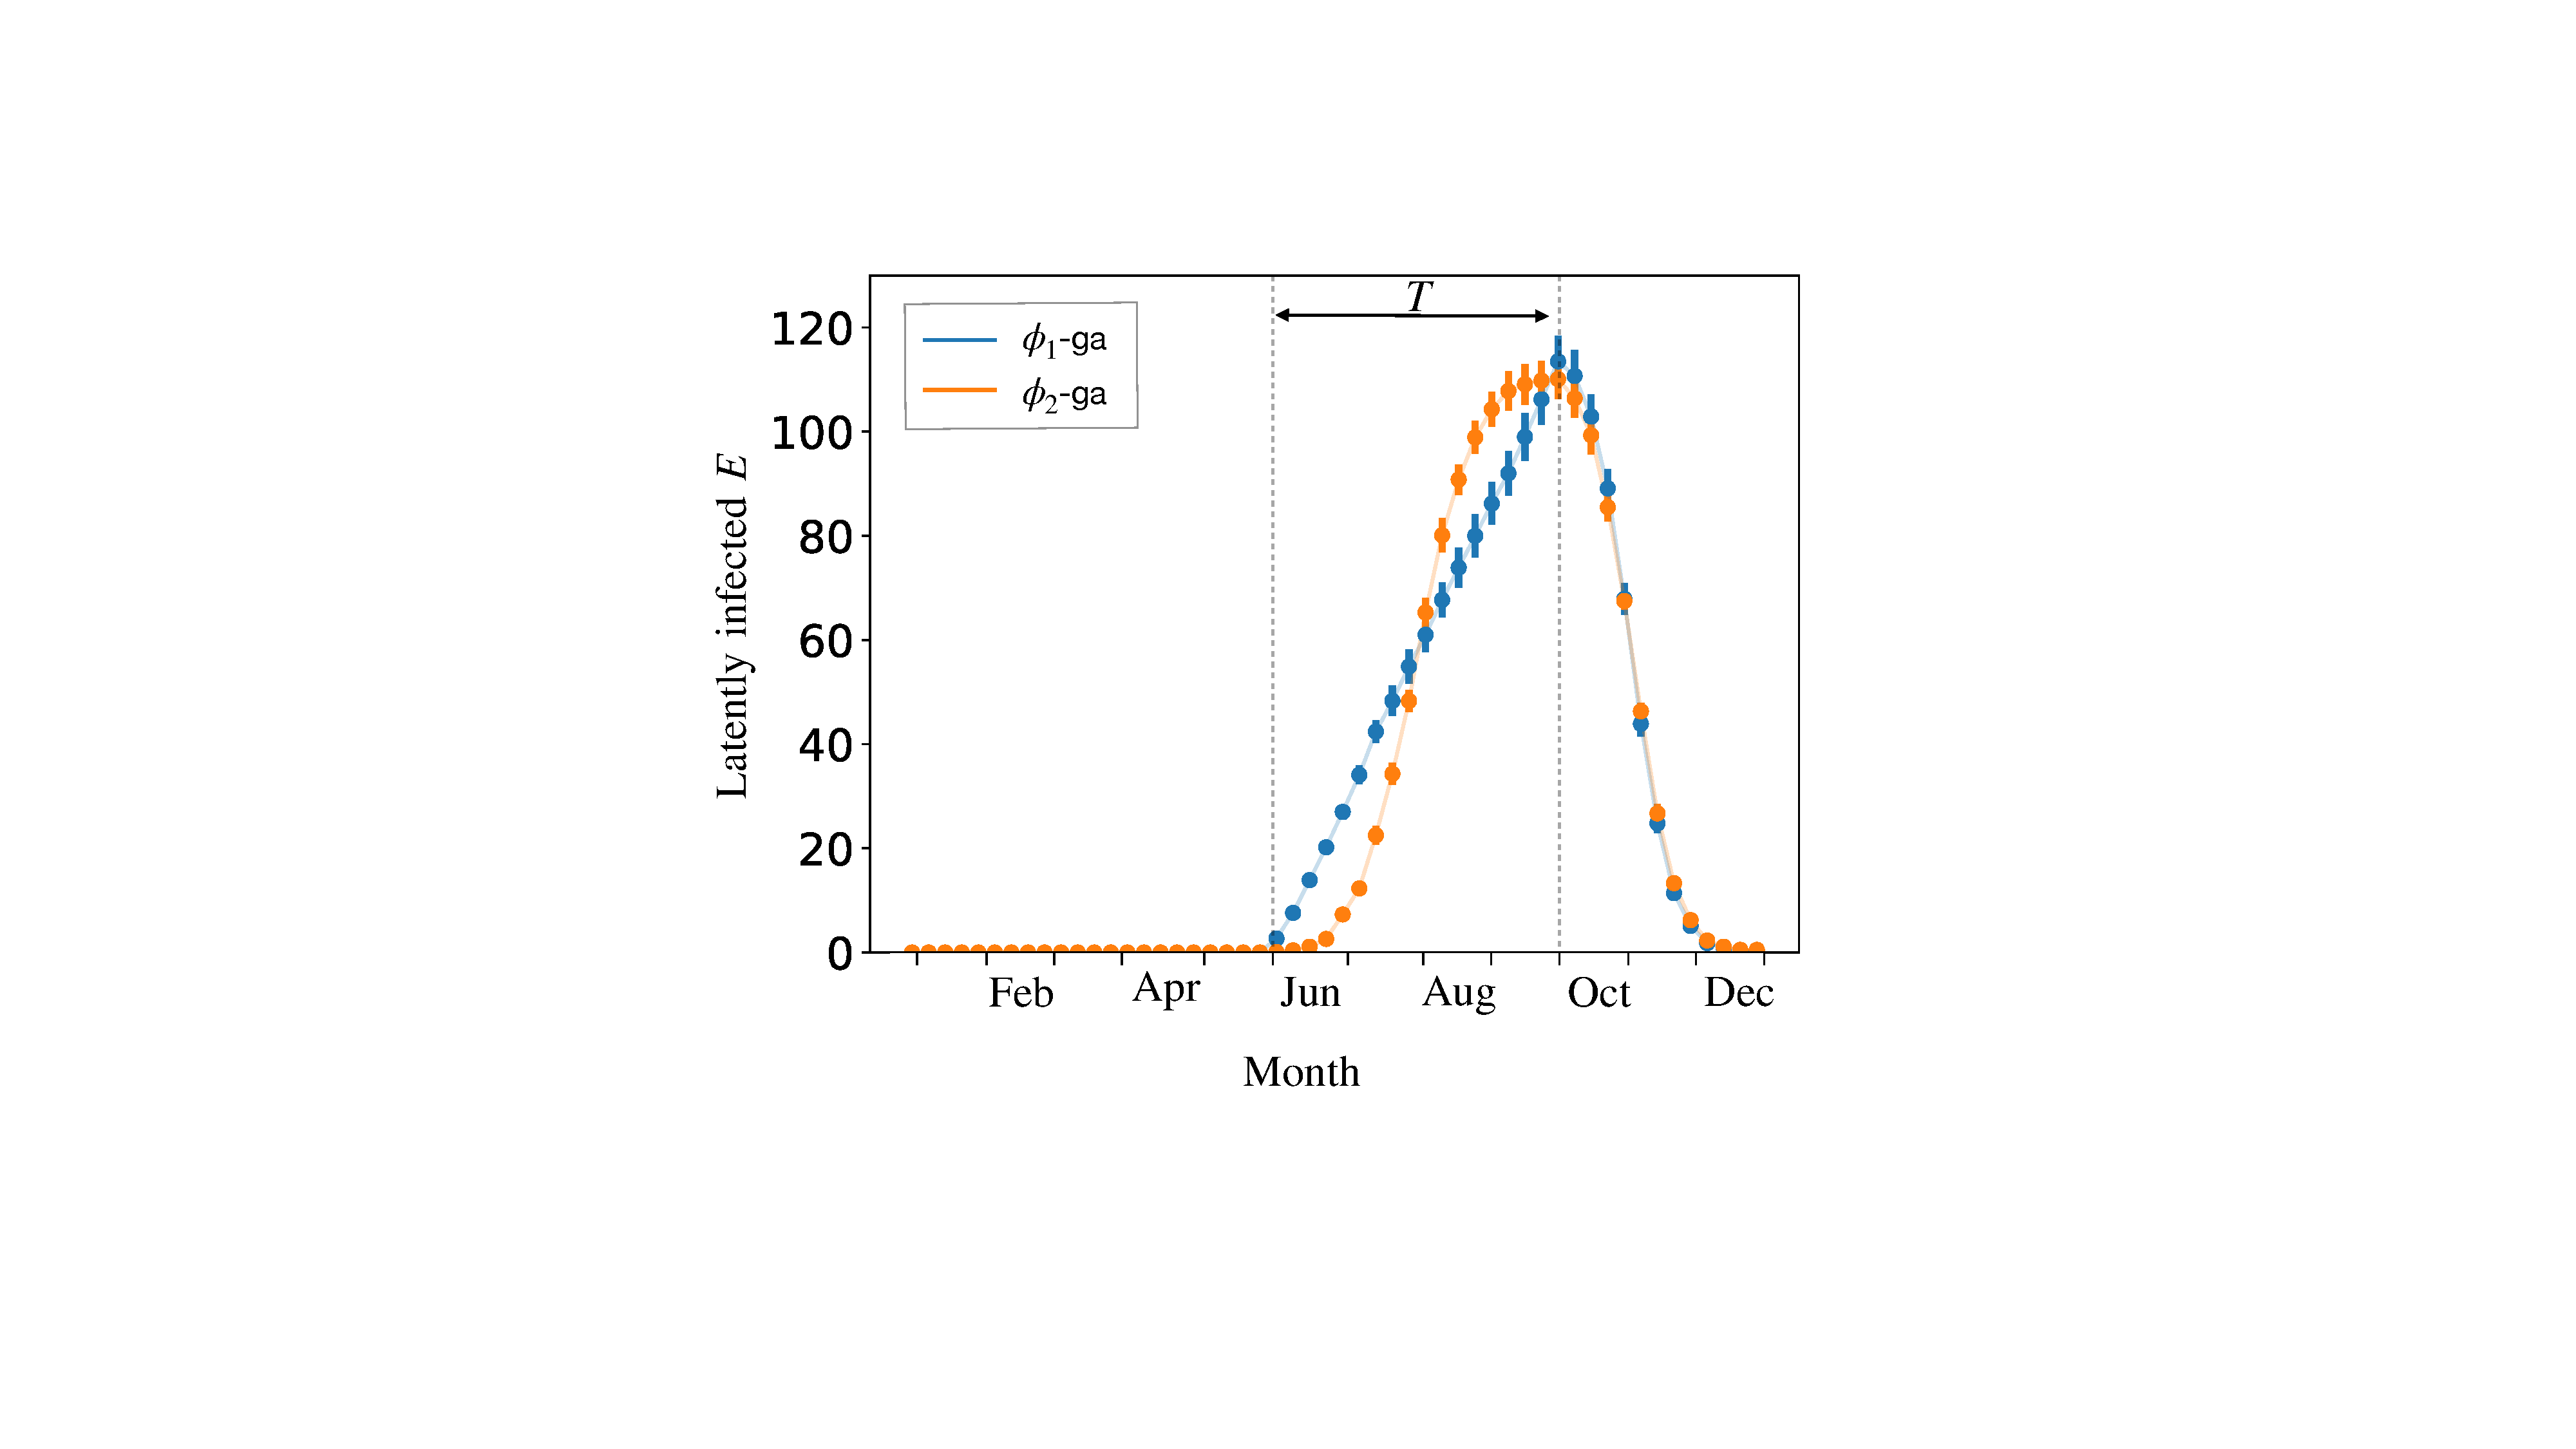
\includegraphics[scale=0.45]{chapter6/figures/fig5-sporulation.pdf}
    \caption{Two year simulations of the power law dispersal model are shown for the sporulation functions $\phi_1(t)$ and $\phi_2(t)$, (a) and (b) respectively.}
    \label{fig:SEIR-sporulation}
\end{figure}


\section{Defining an $R_0$}

Before the $SEIR$ model can be investigated, a measure of the pathogens ability to invade must be defined. For epidemic systems, this usually comes in the form of a reproduction number $R_0$. There are, however, various challenges involved in defining $R_0$ when there are dispersal-mediated secondary infections and spatial structure, as explored in chapter \ref{ch5:dispersal-model}. Chapter \ref{ch5:dispersal-model} demonstrated that $R_0$ is a spatiotemporal function of various epidemiological parameters, and measuring $R_0$ over different spatiotemporal scales can lead to different, and sometimes misleading, results for $R_0$; for a seasonal-based pathogen such as ADB, additional factors only complicate the definition. 

\textit{From this point on, unless otherwise sated, the method for calculating $R_0$ will refer to the average number contact traced secondary infections for each generation of infection, as per Definition \ref{def:R0_contact_traced}. However, this time, secondary infections characterise the transition $S\rightarrow E$ and successive generations of infected ash arise seasonally during sporulation.}

As demonstrated in chapter \ref{ch5:dispersal-model}, a suitable spatial and temporal scale must be chosen to measure $R_0$. Figure \ref{fig:SEIR-R0-definition} shows the contact-traced $R_0$ for the inverse power law model $SEIR$ spreading above the threshold\footnote{The Gaussian variant of the $SEIR$ model also follows the same characteristic decline in $R_0$ for each subsequent generation, as demonstrated in chapter \ref{ch5:dispersal-model}}. For the particular combination of pathogen parameters shown in Figure \ref{fig:SEIR-R0-definition}(a), $R_0$ saturates to around $4$ and there is little difference in measuring $R_0$ between $10, 15$ and $20$ years. Although, measuring $R_0$ over a five year is slightly below the $10-20$ year average. This behaviour is also reflected in Figure \ref{fig:SEIR-R0-definition}(b) where $R_0$ for the first generation infected ash saturates at around $R_0 = 4$. On average, we would expect to see more infectious pathogens saturate faster and less infectious pathogens take longer\textemdash see Appendix \ref{fig:a-R0-saturate}.

\begin{figure}
    \centering
    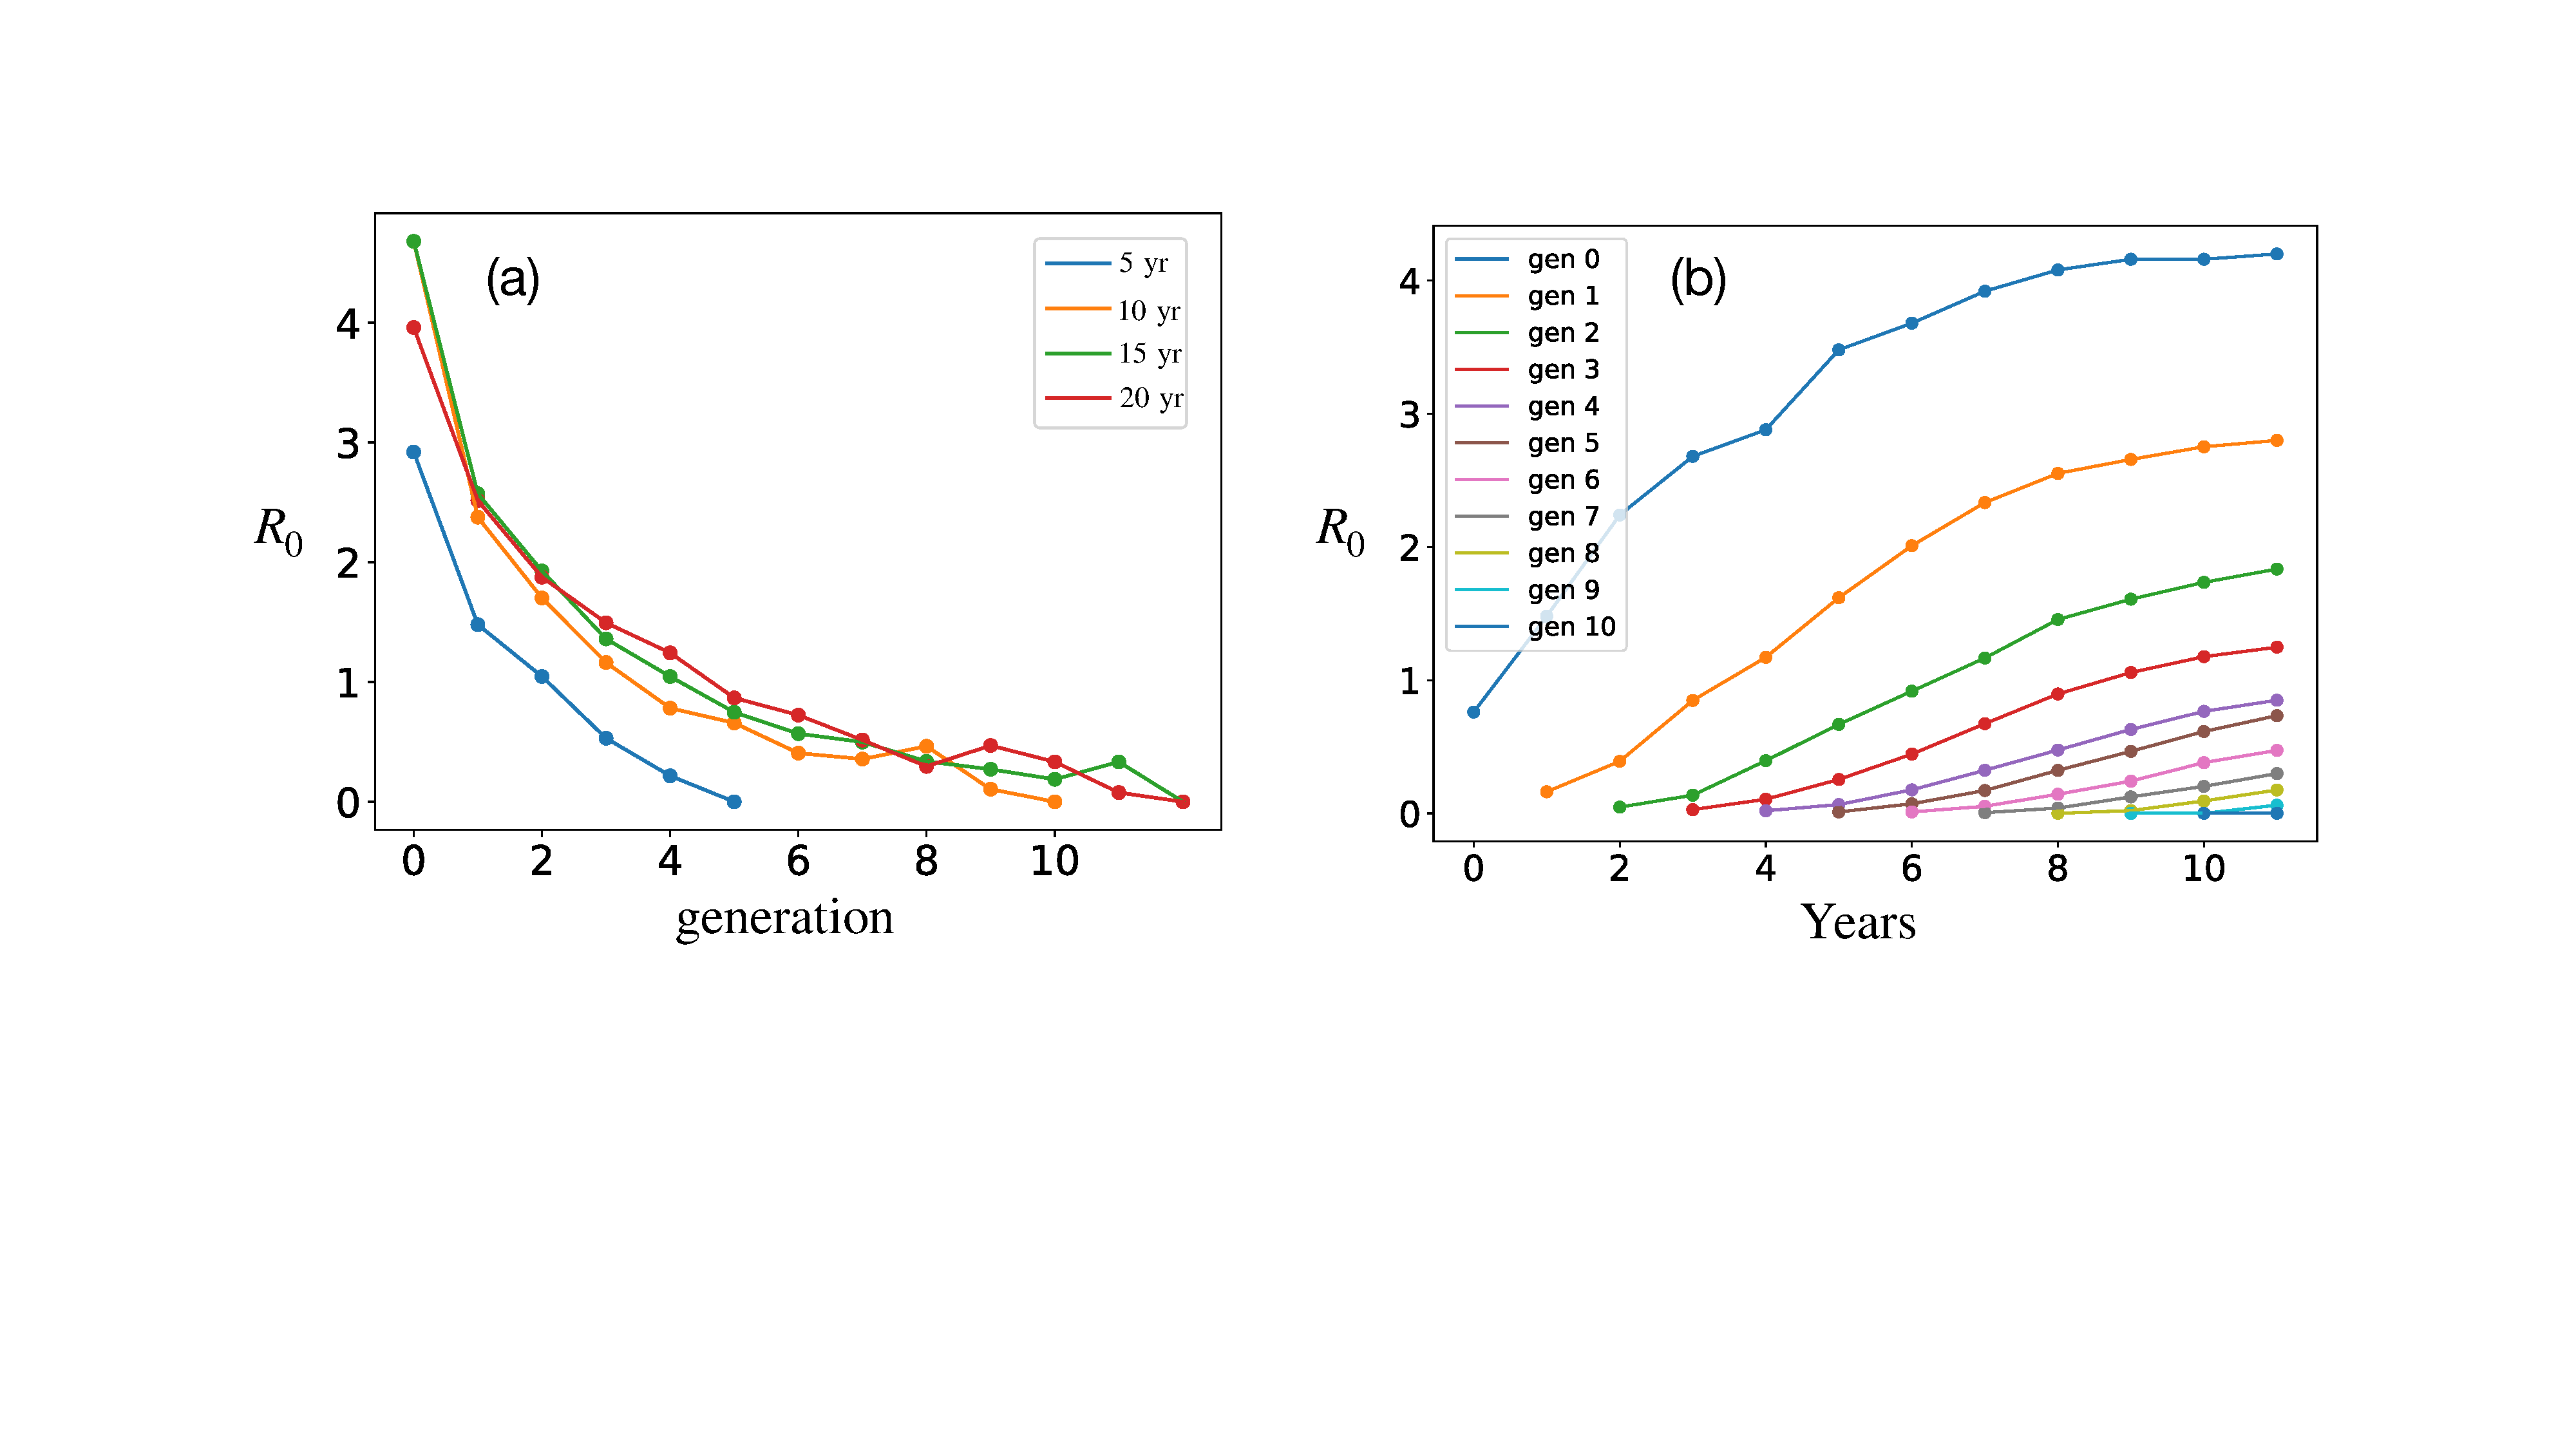
\includegraphics[scale=0.3]{chapter6/figures/fig5-R0-def.pdf}
    \caption{Contact-tracing $R_0$ in the seasonal $SEIR$ model. (a) The average number of secondary infections are shown for ash infected in the $n^{th}$ generation after outbreak (b) The average number of secondary infections is shown against the years after outbreak for different generations $0-10$.}
    \label{fig:SEIR-R0-definition}
\end{figure}

From Figure \ref{fig:SEIR-R0-definitio}(a-b) we can see the familiar saturation of $R_0$ for later generations. The decline in $R_0$ with each generation can be understood by the decline in susceptible ash with time. The first generation infected ash, at $t=0$, have a higher number of susceptible neighbours available to infect, which declines in time. The saturation point of $R_0$ mirrors the infectious lifetime which, in this model are taken to be exponentially-distributed with mean $\lambda=5\ \mathrm{yr}$. In light of better data, this choice of distribution and parameterisation could be updated. 

It makes sense to define a measure for $R_0$ based on the first generation of infections, given that the first generation has, on average, a higher $R_0$. Choosing an $R_0$ in this manner gives us an upper-bound of invasiveness, which for control, is better than an under-estimate:

\textit{The results of this, and the proceeding chapter, therefore, are based on the average number of first generation infected ash.}

Lastly, a suitable domain size $5\mathrm{km} \times 5\mathrm{km}$ was chosen to measure the $R_0$ for first generation infected ash over a $10$ year period. Primarily, this choice was taken for two reasons: 1) larger domain sizes beyond $5\mathrm{km} \times 5\mathrm{km}$ incur increasingly larger computer run times 2) there is little dependence of $R_0$ at, or beyond, this domain size or most values of $\beta$. Although, as shown in Appendix \ref{a:seir-with-L}, it is possible to under-estimated $R_0$ for high values of $\beta$, albeit slightly.

% - Show three different values of beta, above below and at threshold, for ga vs pl 

%\subsection{Defining an R0 value}
% Show that R0 A) over the season B) the problem policy makers experience by not having 5 years to wait before estimates of R0 C) How to form a crude estimate for R0 based on the first season 

% \subsection{Towards $\beta$ parameter-matching}
% - using mortality/infection \% data over match beta against percentage infected

% \subsection{Persistence}
%  - use a 10 year simulation below seasonal threshold, to show that the pathogen can survive for long periods within an area


% discuss multiple sporulation functions

% A simple time-dependant function $\phi(T)$ takes the value of $1$ between the summer months of June - September, and $0$ otherwise thus reflecting the sporulation peak of \textit{Hymenoscyphus fraxineus} (HF). During these summer months, wind-borne dispersal occurs when fruiting bodies produce large numbers of ascospores. 

\section{Informed ash host distribution}

Up to this point, a thorough description of the host data set has been omitted. Ash densities are parameterised by modelled ash abundance data provided by \cite{hill.data}. The canopy cover datasets produced by \cite{hill.data} combine a number of different data sources that cover parts of Great Britain, regression methods are then used to extrapolate canopy cover over the whole of Great Britain\footnote{Previously in chapter chapter \ref{fig:ch4_uk_spread}, the oak canopy cover dataset given by \cite{hill.data} was used in conjunction with the SLM toy model; the insights from doing this then motivated the construction of a generic $SIR$-based dispersal model in chapter \ref{ch5:dispersal-model}.}. Conveniently for the present chapter, ash happened to be among the most accurate data sets given by \cite{hill.data}. For a more in-depth description of the methods used by \cite{hill.data} and a review of host data in general, see chapter \ref{chapter:lit-rev}.

\begin{figure}
    \centering
    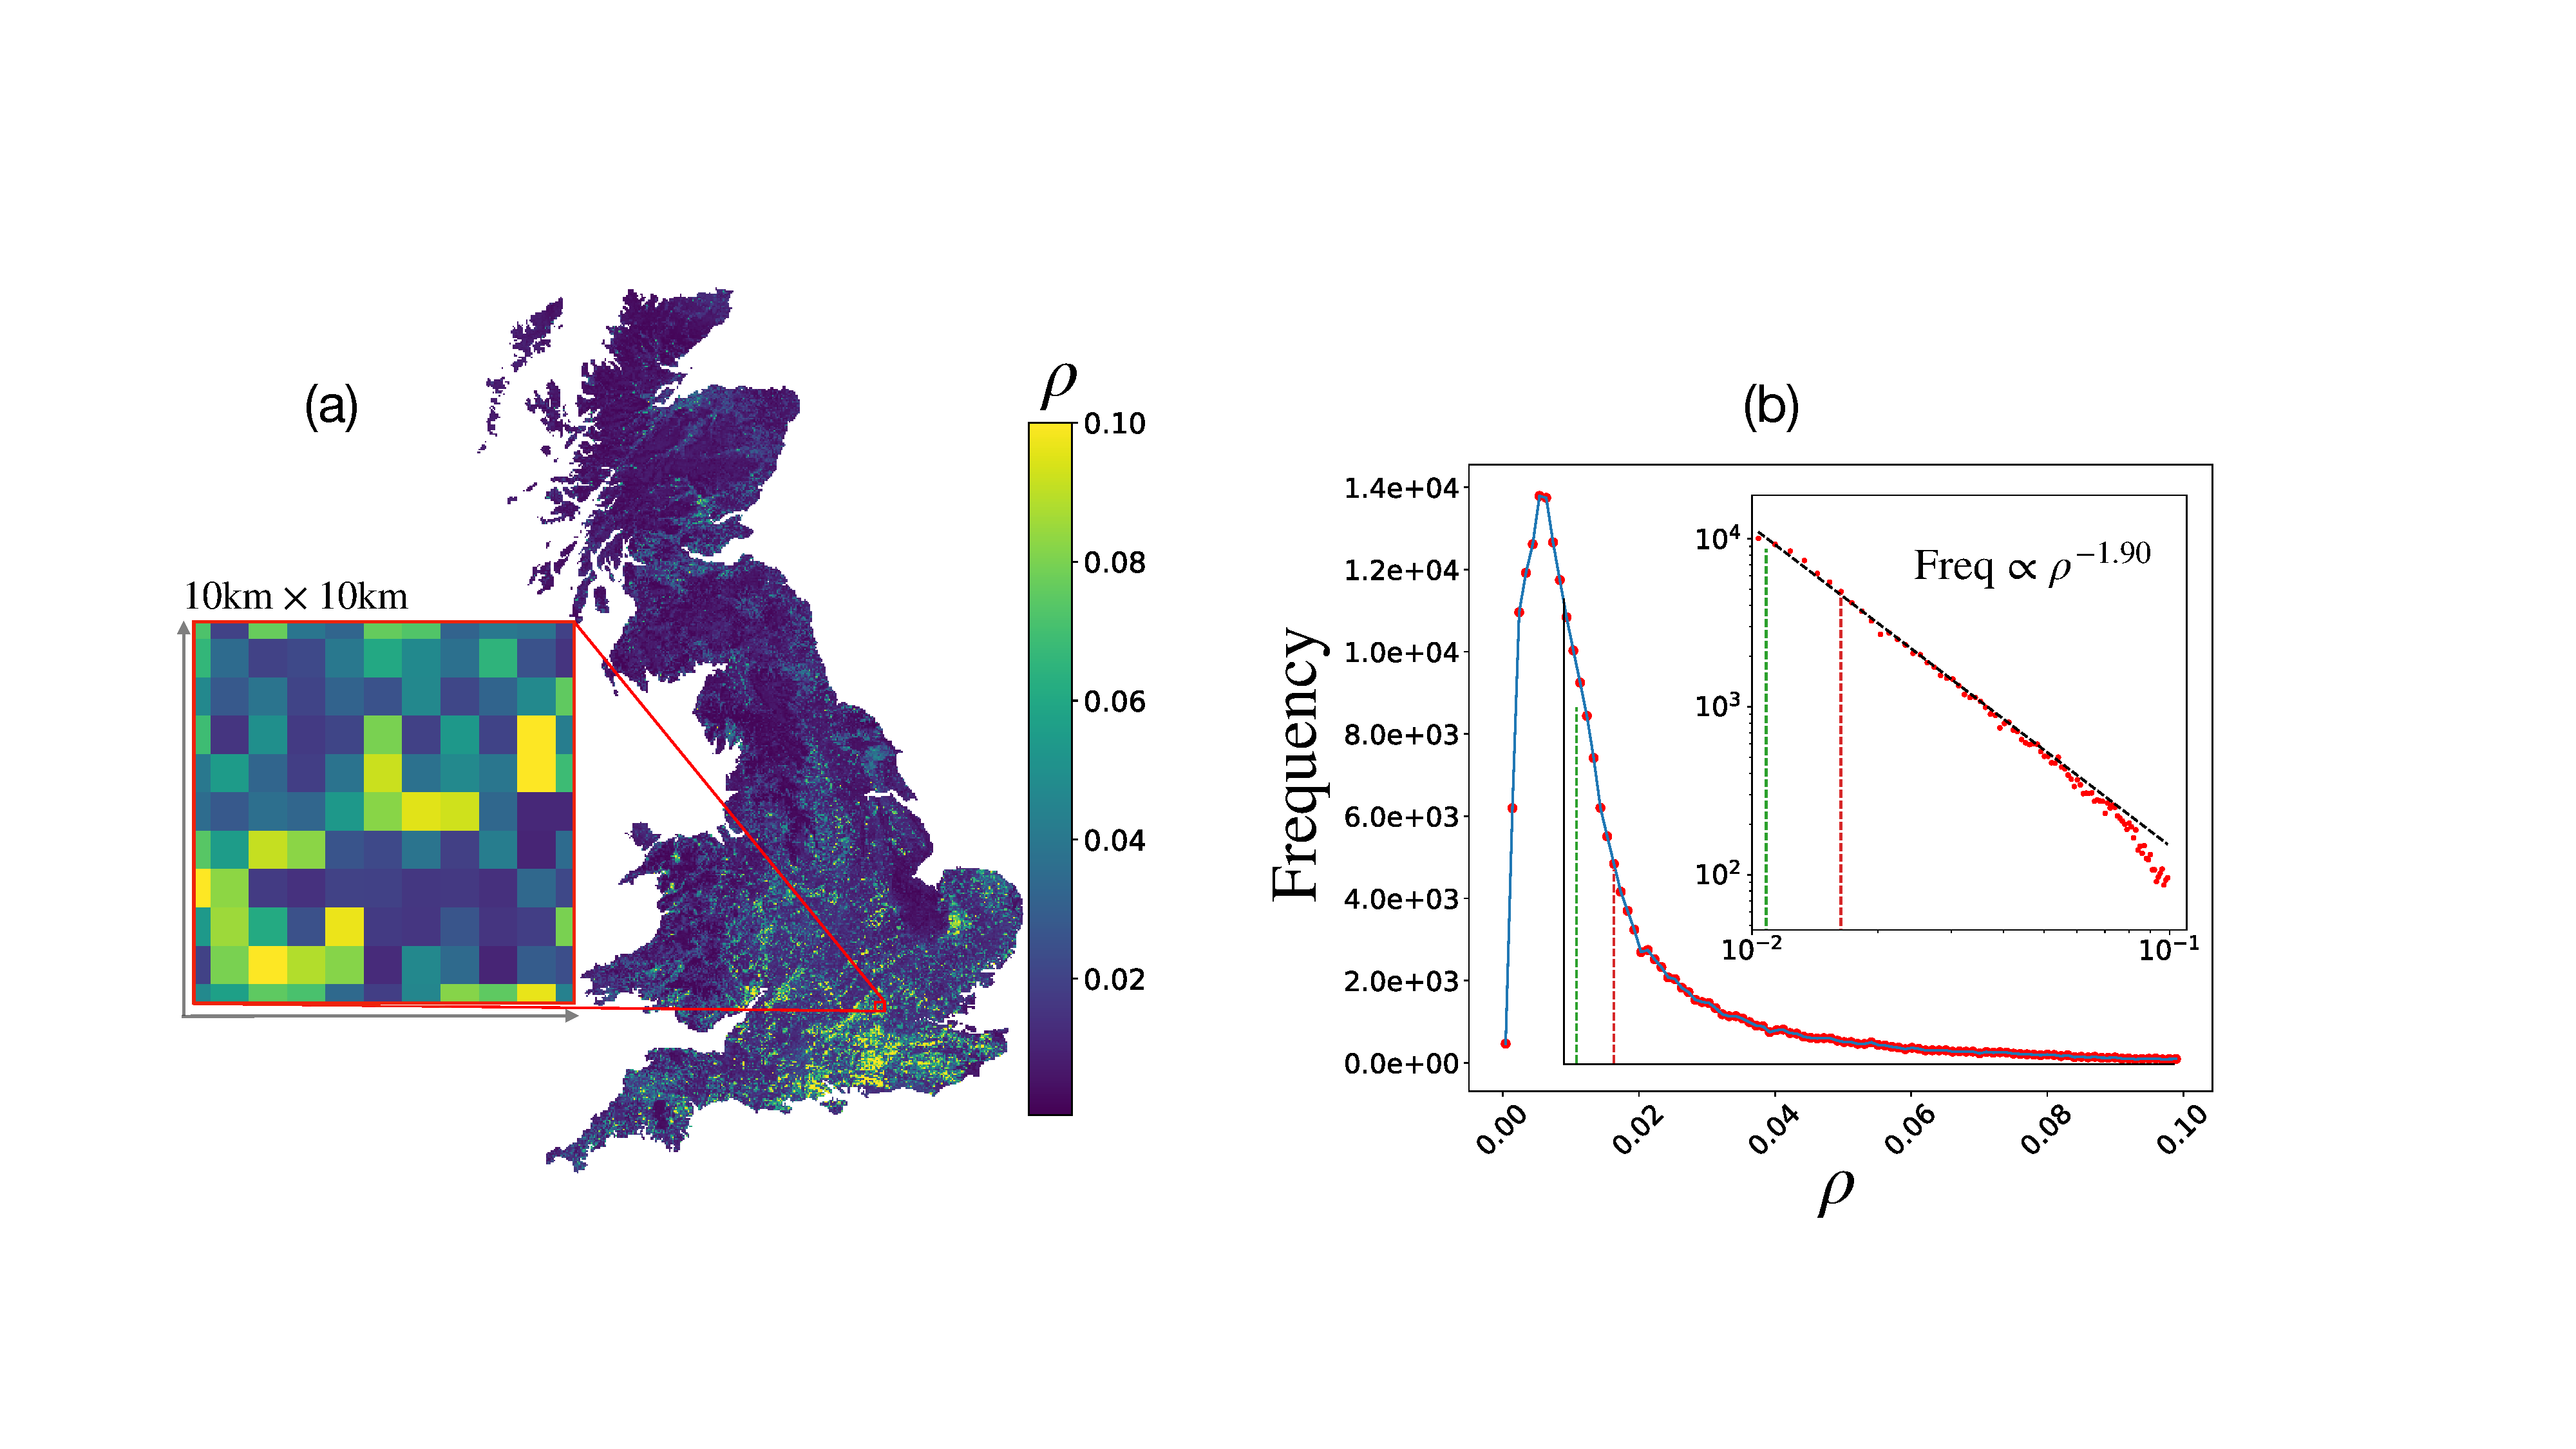
\includegraphics[scale=0.30]{chapter6/figures/fig3-ash-data.pdf}
    \caption{Ash canopy cover data, as modelled by \cite{hill.data} converted into a density. (a) a map of ash densities at a resolution of $1\mathrm{km} \times 1\mathrm{km}$ (b) the distribution of ash density over Great Britain, the inset shows a inverse power law behaviour.}
    \label{fig:ash-host-data}
\end{figure}

Figure \ref{fig:ash-host-data}(a) shows a density map of ash, at a resolution of $\mathrm{1km}\times \mathrm{1km}$, produced from abundance data given by \cite{hill.data}. From Figure \ref{fig:ash-host-data}(a), the south of England contains the highest concentration of high-density ash patches and ash become progressively less abundant in Scotland and coastal locations, in western Whales for example. A higher density of ash can be expected to yield a higher number of secondary infections, in line with the results of chapters \ref{ch3:two-param-model}-\ref{ch5:dispersal-model}.
 
The frequency distribution is shown in Figure \ref{fig:ash-host-data}(b) and reveals that the average density of ash in Great Britain is $\rho=0.017$ and that few locations support densities of $\rho=0.10$ and over\footnote{In the original $2.2\times 10^4$ $1\mathrm{km^2}$ data points, there were a handful of outlier points with densities in the interval $\rho \in [0.10, 0.30]$ which were excluded from the analysis.}. Between the limits of $\rho \in [10^{-2}, 10^{-1}]$, the frequency distribution in Figure \ref{fig:ash-host-data}(b) follows a power law of the form $\sim \rho ^{-k}$, as evident from the linearity on the logarithmic inset axes. The distribution had a fitted exponent of $k=1.90$, shown by the dashed black line. Intriguingly, this observation is suggestive of self-similarity in the data.

Two modifications had to be made to the modelled ash canopy cover data in order to complement the $SEIR$ model. Firstly, the raw abundance values were re-scaled into a dimensionless tree density $\rho$. The same process was outlined in chapter \ref{ch5:dispersal-model} i.e. by converting the units $\mathrm{ha/km^2}$ to kilometre-squared of ash cover per kilometre-squared of land. Secondly, the map resolution has to be re-scaled to reflect the intrinsic spatial scale of local wind-borne dispersal, this topic is resumed below in section \ref{ch6:re-scaling-host-data}, when ADB $R_0$-maps are constructed over Great Britain.

\section{Constructing $R_0$-maps over Great Britain}

In this section, $R_0$ values of the $SEIR$ model of ADB will be projected onto the host distribution of ash, given by \cite{hill.data}, to create $R_0$-maps. Doing so will permit the investigation of a novel control strategy. But first, to accurately project $R_0$ values onto the host distribution, the spatial and temporal scale of pathogen transmission in the $SEIR$ model must be made to match the domain resolution and the infectious lifetime of the pathogen, respectively. This requires a re-scaling of the host distribution.

\subsection{Re-scaling the host distribution}
\label{ch6:re-scaling-host-data}

A choice was made to re-scale the pixel size of ash density in Figure \ref{fig:ash-host-data}(a), from $1\mathrm{km} \times 1 \mathrm{km}$, to $5\mathrm{km} \times 5 \mathrm{km}$. In the local scale field study conducted by \cite{grosdidier2018tracking}, fungal spores were detected at a maximum distance of $500\mathrm{m}$ away from a known source of infection. So on the surface, the original $1\mathrm{km} \times 1 \mathrm{km}$ resolution of the abundance data, as reported by \cite{hill.data}, appears reasonable. However, with moderate-high values of $\beta$ the power law $SEIR$ model demonstrates that singular jumps can exceed $1\mathrm{km}$ and since we cannot know $\beta$ for sure, it is desirable to air on the side of caution and re-scale the domain such that pixels represent larger spatial areas. In doing so, the resolution is lowered along with the level of spatial-structure. 

\begin{figure}
    \centering
    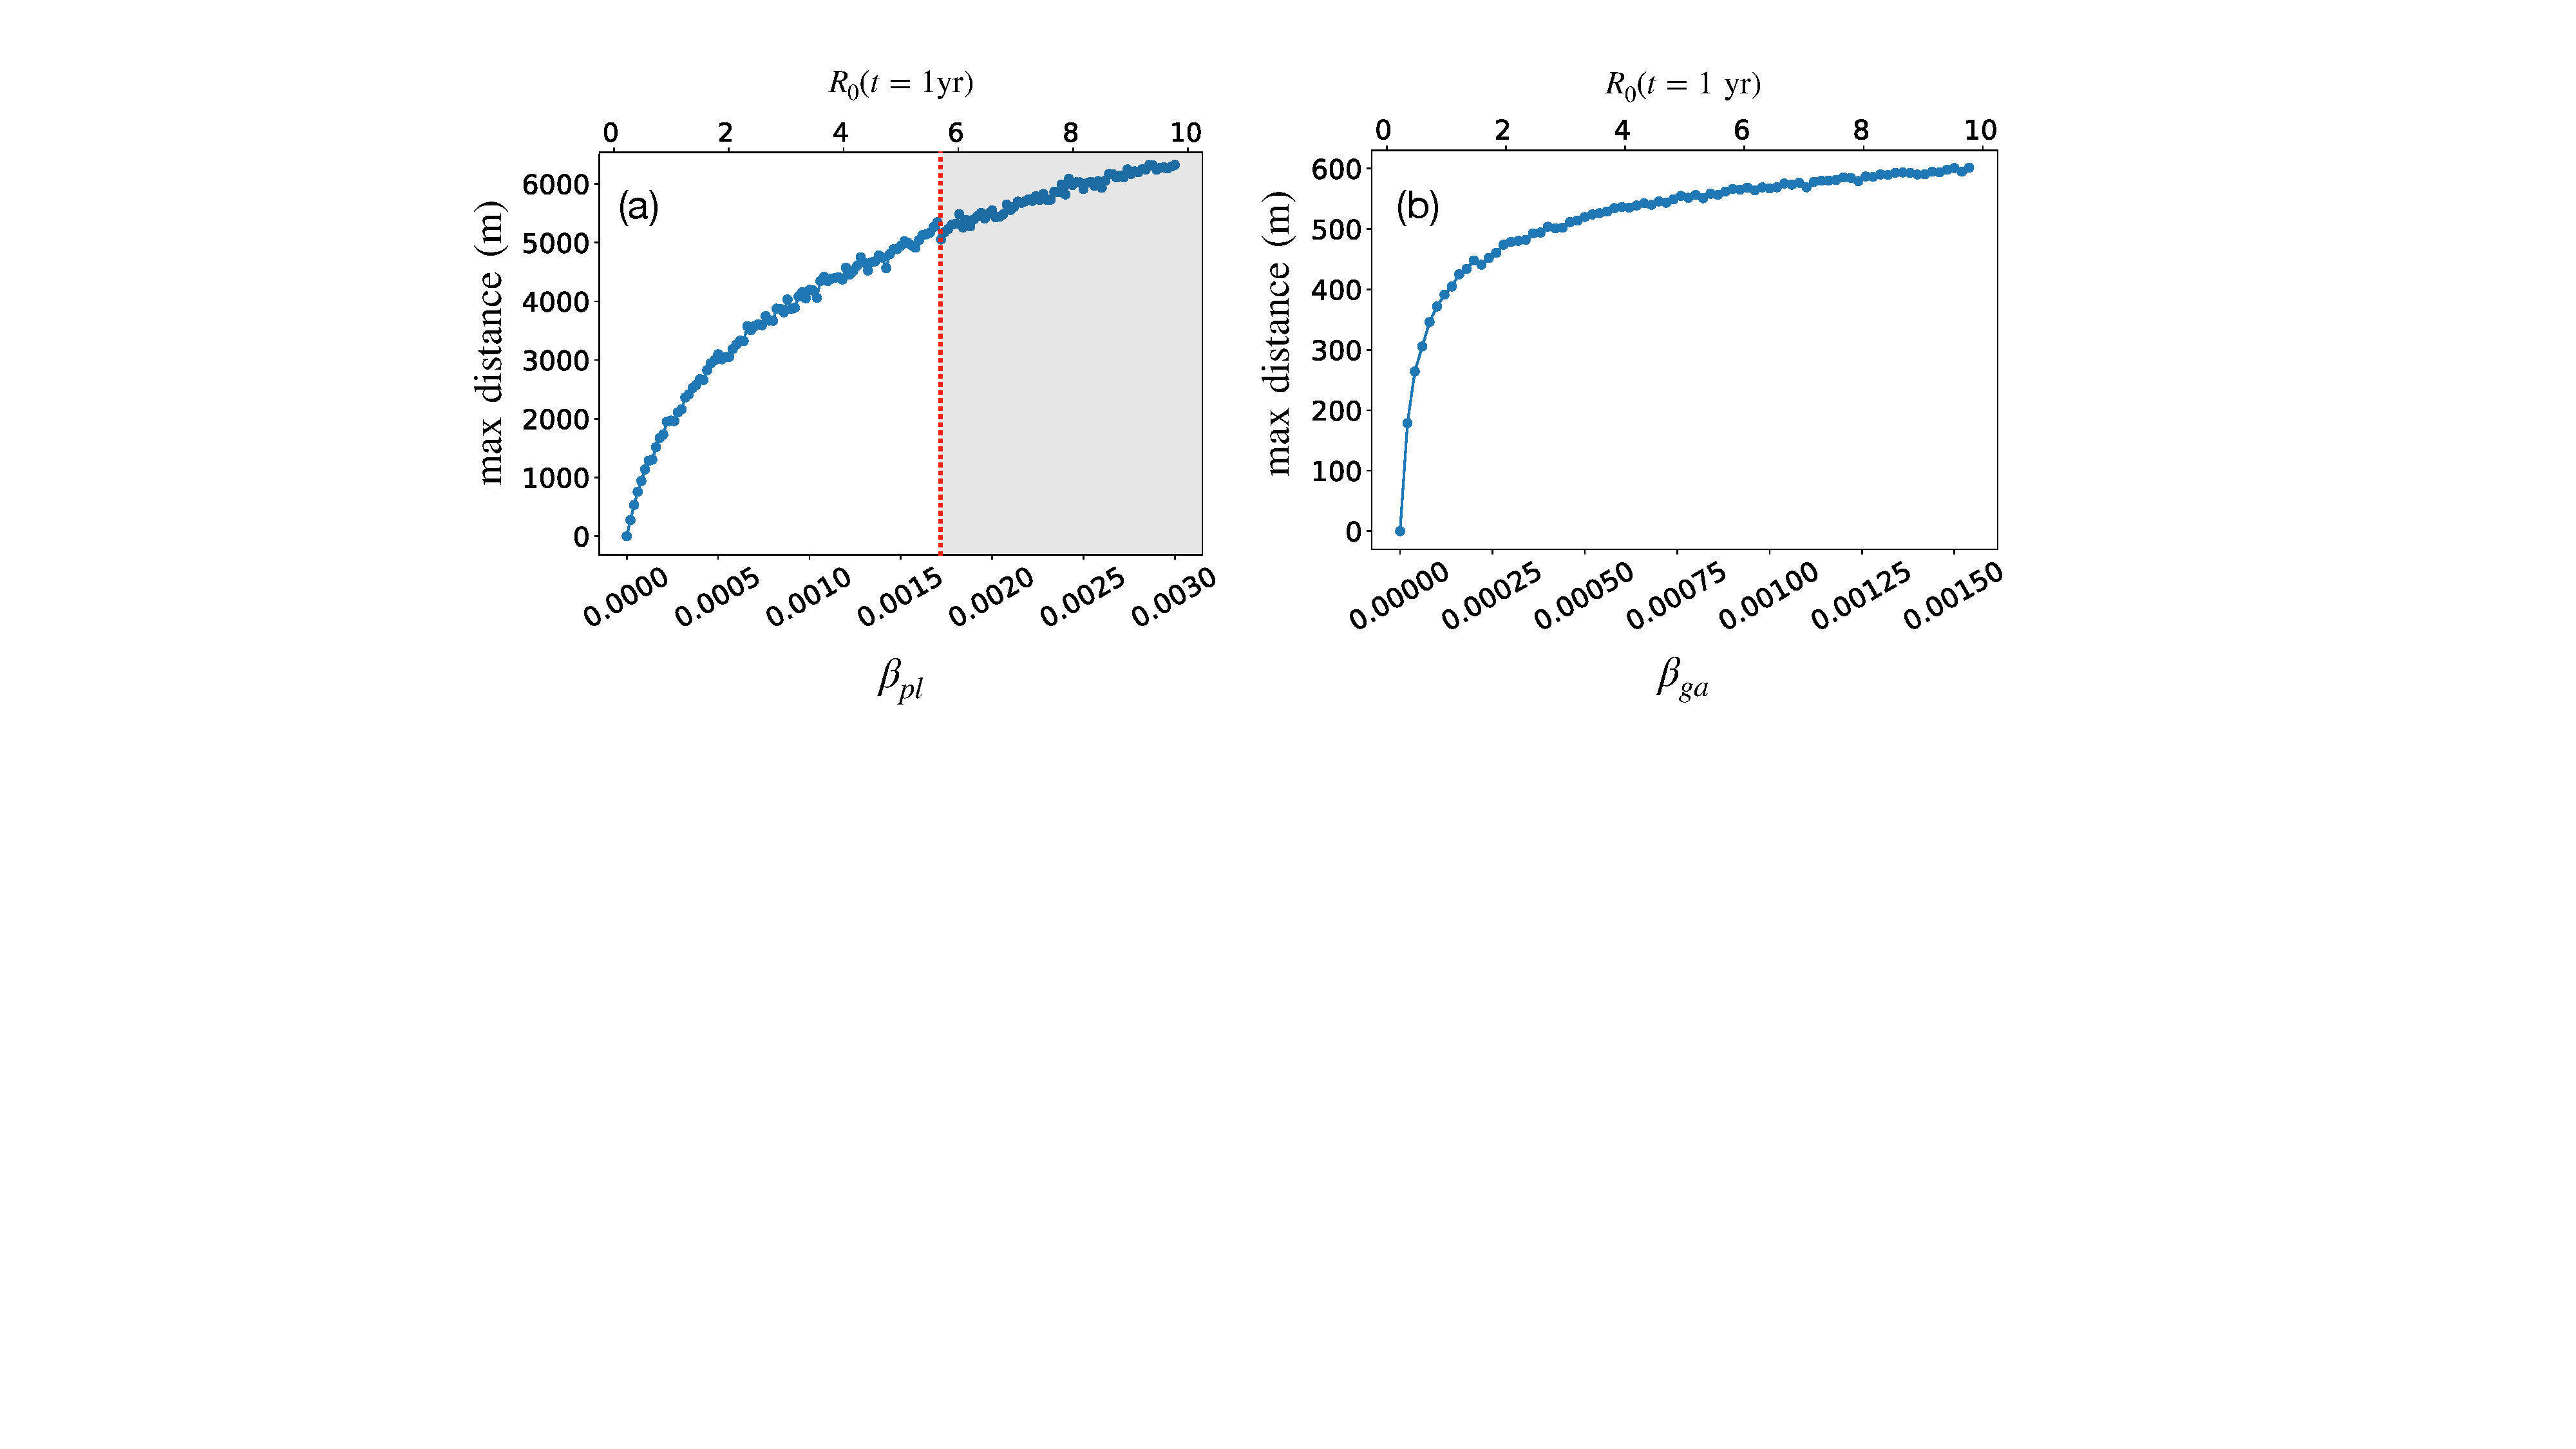
\includegraphics[scale=0.40]{chapter6/figures/fig5-beta-vs-max_d.pdf}
    \caption{The maximum distance that can be be traversed by the pathogen in a single jump is shown against different values of $\beta$. (a) the inverse power law based dispersal (b) the Gaussian dispersal.}
    \label{fig:max_dist_vs_R0}
\end{figure}

Suppose two patches of land, having tree densities above the threshold, $R_0 = 1$, are separated by an intermediary patch below the threshold. If we are not careful, dispersal could traverse the below-threshold patch within a single jump, even at local spatial scales. As such, we must choose a domain resolution that gives some assurance that, at the local scale, wind-dispersed spores cannot jump over whole patches with singular jumps. As always, there is the possibility that spores disperse more considerable distances, from mainland Europe to Great Britain, for example, \cite{freer2017tree, wylder2018evidence}. Nevertheless, this chapter aims at targeting dispersal at local scales, and LDD can be omitted for now.

Ensemble simulations can measure the maximum dispersal distance by averaging the maximum distance of secondary infections. Figure \ref{fig:max_dist_vs_R0} shows of the maximum distance traversed by the pathogen for different values of $\beta$ over a large domain, $20\mathrm{km^2}$, in a single year\textemdash or jump. The ensemble simulations shown in Figure \ref{fig:max_dist_vs_R0} start from a small number of infected trees at the centre of the domain and contrast the difference between inverse power law and Gaussian models\footnote{This is indicated by the difference in subscript on $\beta$. Technically, both are models in their own right, so a comparison between both of them with the same value of $\beta$ does not make sense. Although both models cannot be compared directly, insight can be gained by comparing model behaviours over the same $R_0$ axis.}, (a) and (b) respectively. 

Interestingly, dispersal in the Gaussian model can be seen to level off between $500-600\mathrm{m}$ in line with the results from \cite{grosdidier2018tracking}, whereas, for power law dispersal, dispersal continues to rise. No doubt, this observation reflects the thin-tailed Gaussian and fat-tailed inverse power law dispersal kernels. For the exact value of $R_0$, inverse power law model can be seen to travel much further than Gaussian model and echos the difficulty of controlling fat-tailed dispersal \cite{WEBIDEMICS}, and more broadly, LDD.

For a $5\mathrm{km} \times 5 \mathrm{km}$ host distribution, we can therefore place an upper limit on $\beta$, indicated by the shaded region in Figure \ref{fig:max_dist_vs_R0} (a). If an infectivity parameter surpasses $\beta = 0.0016$, the pathogen has potential to jump over $5\mathrm{km} \times 5 \mathrm{km}$ patches and infect non-nearest neighbours. In this scenario, patches either need to be re-scaled to larger values, or the neighbourhood of interaction made non-local, as in \textcolor{red}{cite non-local R0 maps, Gilligan.} Fortunately for us however, the reproduction ratio of $R_0=6$, shown in Figure \ref{fig:max_dist_vs_R0} (a) indicates that infectivity parameters of $\beta = 0.0016$ and above are likely too high\footnote{\textcolor{red}{The value of $R_0$ shown in Figure \ref{fig:max_dist_vs_R0} (a) was measured over one sporulation season. If $R_0$ for this value of $\beta$ was measured over the mean life-time of an infected tree, we could expect to see exceedingly high, and probably unrealistic, values of $R_0$. To put this into context, the highest known case of $R_0$ is measles that...}}.

\subsection{Tree density and $R_0$}

The relationship between $R_0$ and tree density $\rho$ is shown in Figure \ref{fig:R0-map-generation}(a) \textcolor{red}{for all four $SEIR$ variants, i.e. the different dispersal kernels and sporulation functions. Conveniently, all $SEIR$ implementations retain the same linearity as the generic $SIR$ model, as explored in chapter \ref{ch5:dispersal-model}}. The regime of pathogen extinction is shown in shaded grey along with vertical  lines that correspond to a critical `density threshold' denoted by $\rho_c$ (equivalent to the threshold $R_0 = 1$). When used in conjunction with the data-set from \cite{hill.data}, Figure \ref{fig:R0-map-generation}(a) represents an appropriate projection of $R_0$ over the map of Great Britain.

\begin{figure}
    \centering
    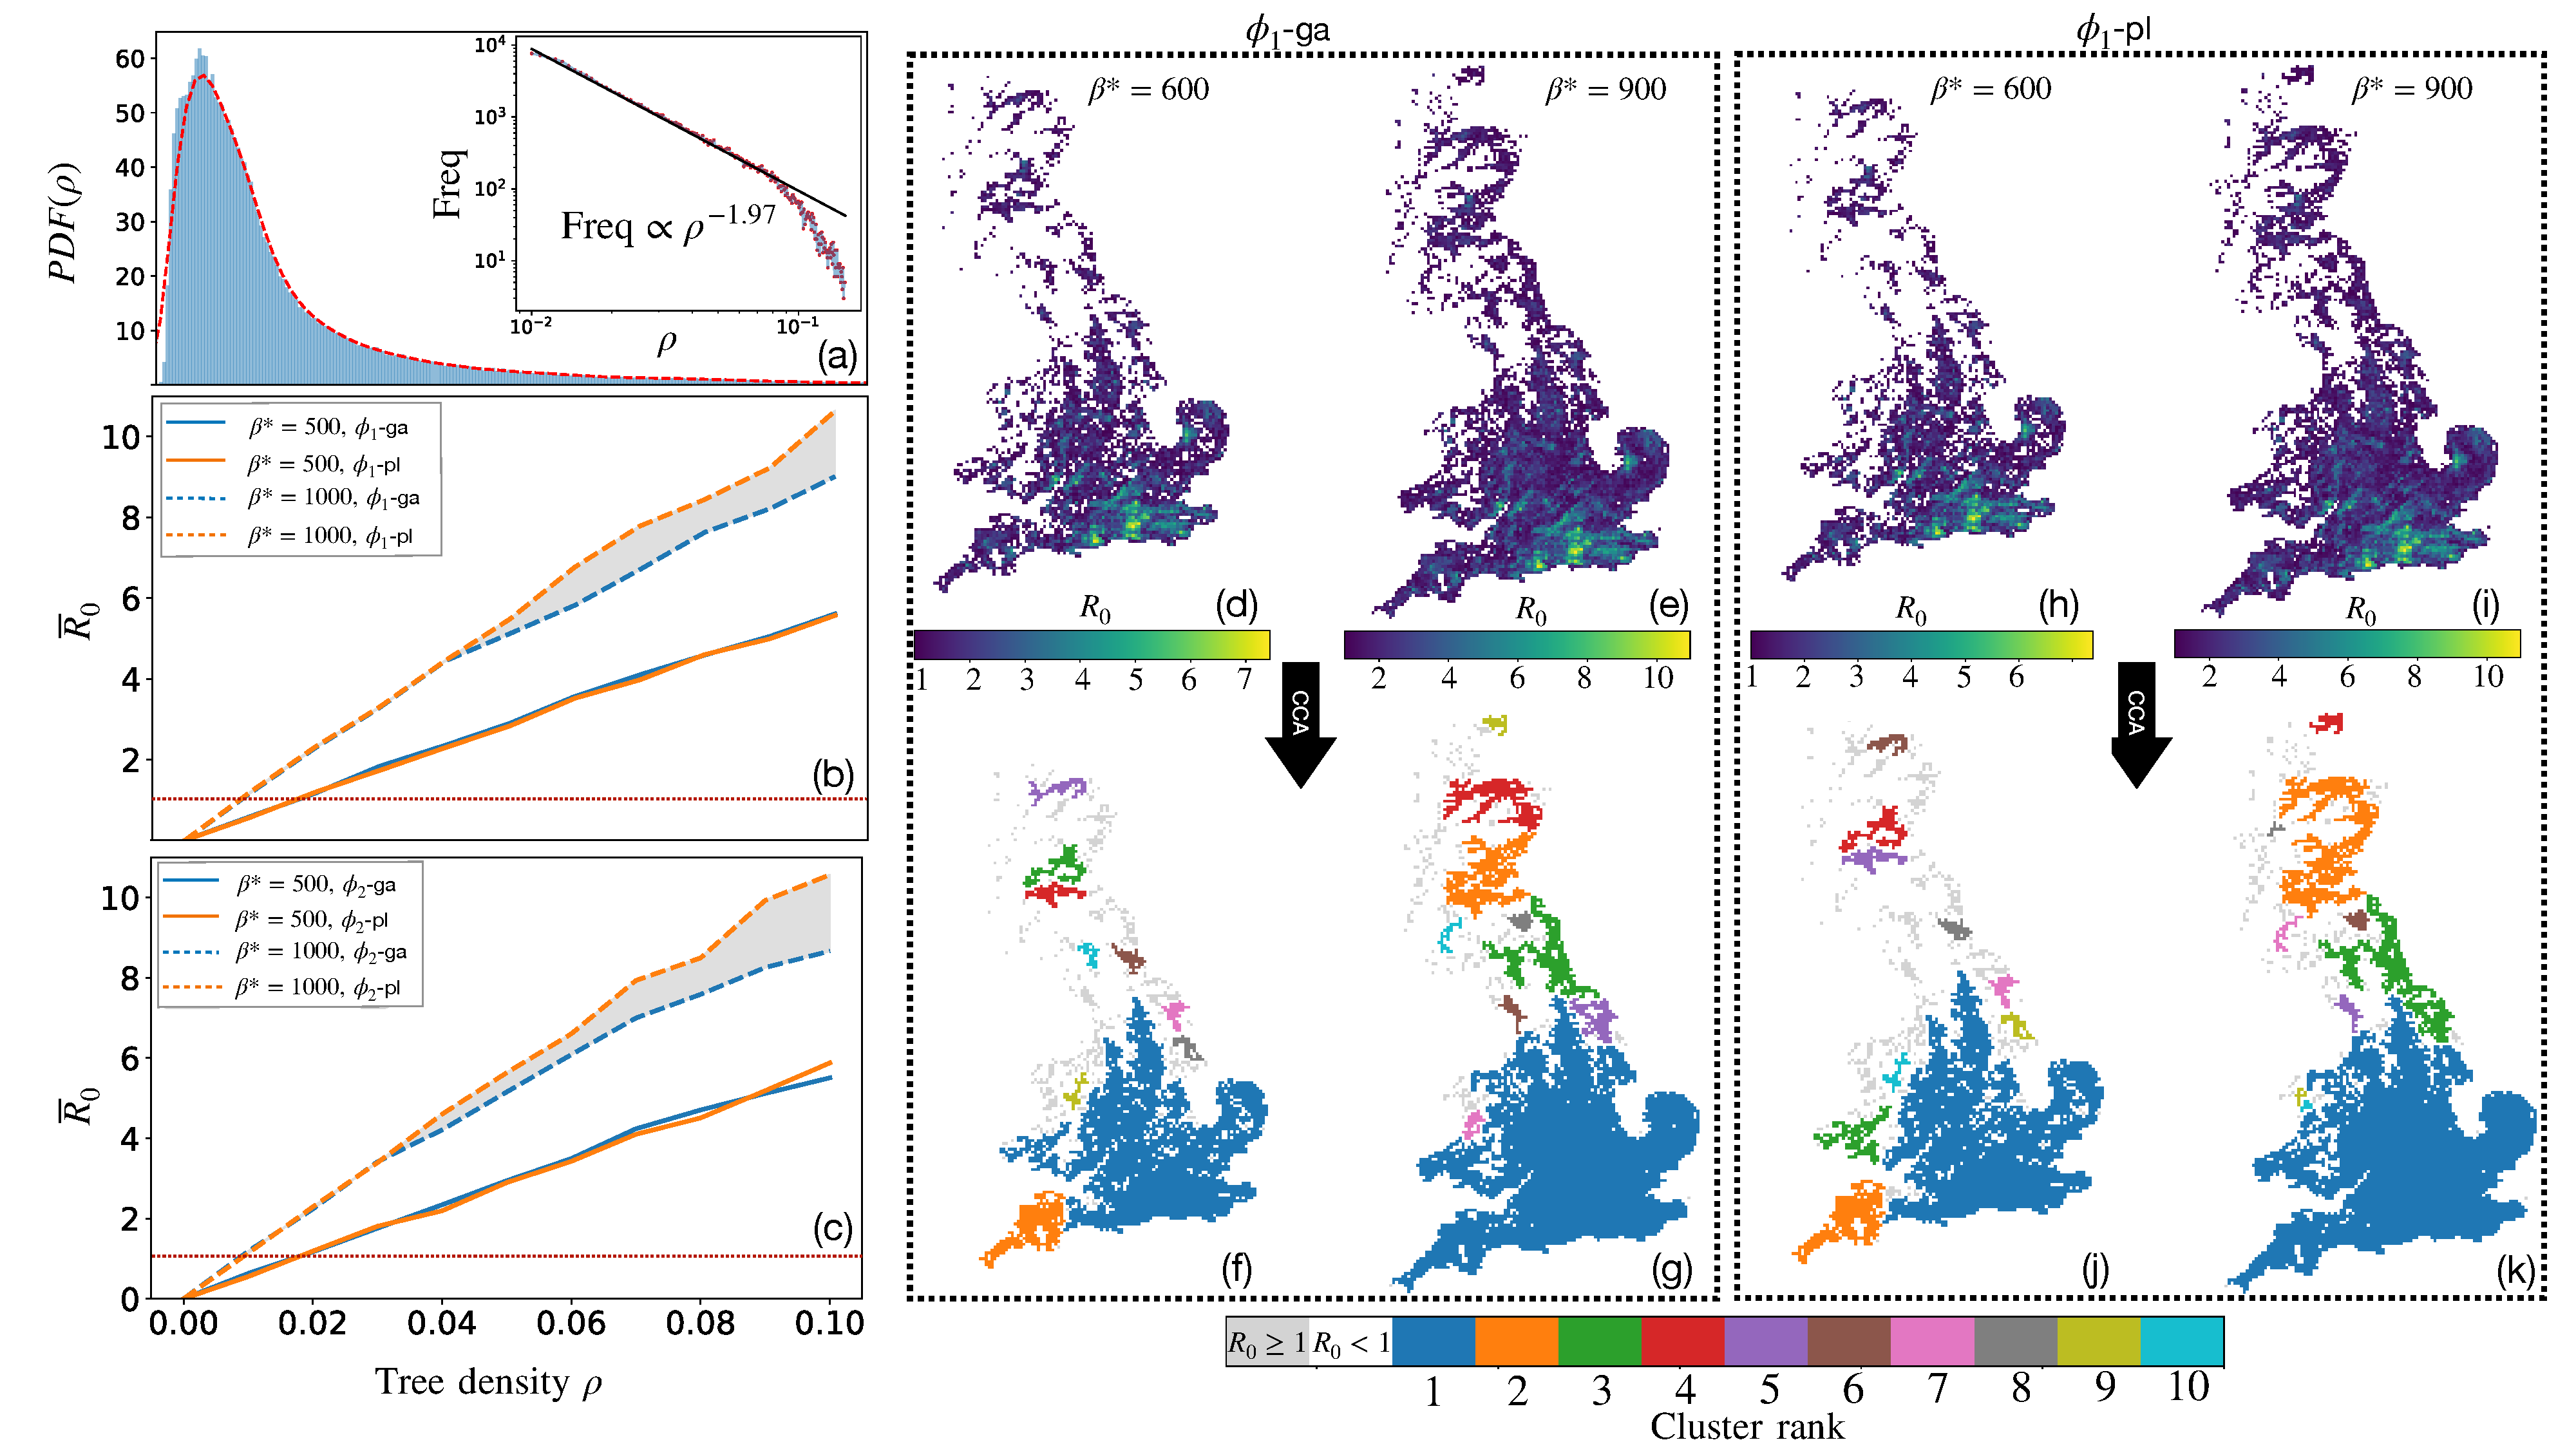
\includegraphics[scale=0.55]{chapter6/figures/fig6-R0-map-generation.pdf}
    \caption{Generating $R_0$ maps for ADB over Great Britain. (a) Ensemble-averaged results of $R_0$ are plotted against the tree densities informed by \cite{hill.data}. (b-c) Projecting $SEIR$ inverse power law $R_0$ values onto the re-scaled $5\mathrm{km} \times 5 \mathrm{km}$ ash host-distribution for two values of $\beta_{pl}$. Patches of land below $R_0 = 1$ are shown as white space. (d-e) The top $10$ largest connected, and susceptible, $R_0$-clusters that are present in maps (b-c).} % in fig (a), include Gaussian and phi(t)_2
    \label{fig:R0-map-generation}
\end{figure}

Figures \ref{fig:R0-map-generation}(b-c) show the reproductive ratios for the inverse power law model projected onto the host distribution of ash. For all variants of the $SEIR$ model, $R_0$-maps look similar, albeit with different $\beta$ values, see Appendix \ref{fig:a-R0-maps-SEIR-variants}. The values of $\beta$ shown in Figures \ref{fig:R0-map-generation}(b-c) correspond to the exact values of $\beta$ shown by blue and orange lines in Figure \ref{fig:R0-map-generation}(a) respectively. Under the influence of a more infectious pathogen, larger areas of the ash population become susceptible by supporting the growth and reproduction of the pathogen, illustrated by the higher density of patches in Figure \ref{fig:R0-map-generation}(c). All locations below the transmission threshold were presumed disease-free and given numerical values of zero, depicted by inland white space. All values of $R_0$ over and above the threshold were taken as susceptible. 

\subsection{Clustering in the $R_0$ map}

We can begin identifying heterogeneity and high-risk clusters of ash by looking at Figures \ref{fig:R0-map-generation}(b-c). However, visualising which pixels connect to form large clusters is non-trivial. An image processing technique, called connected component analysis (CCA) \cite{CCA1, CCA2}, was used to identify and label susceptible clusters and simplify the $R_0$-map. The Python-SciPy package `ndimage' \cite{scipy} was used to implement CCA via the function `label'. Doing so labelled all susceptible neighbours as connected members of the same cluster, according to a structuring element \cite{liang1989erosion}. That is, if two susceptible patches of ash lie within the same neighbourhood, defined by the structuring element, they are connected members of the same cluster\footnote{Structuring elements have their roots in shape and image analysis \cite{23111}, where they define how distinct binary shapes connect to form images \cite{liang1989erosion, nachtegael2001connections}}. More information on structuring elements and CCA can be found in Appendix \ref{a:R0-map-construction}.

Moore and Von-Neumann neighbourhoods were chosen as structuring elements to classify connected components, \textcolor{red}{chapter 3}. Although, for simplicity, the present section is concerned with the Moore neighbourhood\textemdash a comparative look exploring the differences between Von-Neumann and Moore structuring elements is resumed below in section \ref{R0-over-beta}. Figures \ref{fig:R0-map-generation}(d-e) show the top 10 largest $R_0$-clusters, by area, that are present in the $R_0$-maps of Figures \ref{fig:R0-map-generation}(b-d) according to the Moore neighbourhood.
In this simplified interpretation, clusters represent a connected medium of ash capable of supporting an epidemic, whereas regions below the threshold act as natural barriers that inhibit the spread. Therefore, epidemic impact in this model will correlate closely to cluster size, as only large clusters have the potential to support large outbreaks. 

The domain resolution of $5\mathrm{km} \times 5 \mathrm{km}$ ensures that at local spatial scales, pathogen dispersal will not jump directly between clusters but tend to remain localised. Although unlikely, the pathogen may still use intermediary trees inside below-threshold patches of ash as stepping stones and jump between clusters indirectly. Conceptually, this has been described for pathogens jumping between crop fields \cite{Gilligan-disease-management}. \textcolor{red}{This intermediate jumping between cluster is explored more in chapter \ref{ch7:pde} in the context of landscape control.}

At local scales, the epidemic spread within an $R_0$-cluster of ash can be reduced to a `\textit{percolation-like}' problem, with the caveat of heterogeneity. If susceptible patches of ash were homogeneously distributed, a minimum number of susceptible (or `open' in percolation theory) positions would define a critical density, and a spanning cluster would percolate through the domain, as laid out in chapter \ref{ch3:two-param-model}. A similar picture is painted within the $R_0$-maps shown in Figures \ref{fig:R0-map-generation}(d-e). Figure \ref{fig:R0-map-generation}(d) depicts a fragmented domain at $\beta_{pl}=...$, increasing the pathogen infectivity to $\beta_{pl}=...$ yields a much larger '\textit{dominating}' $R_0$-cluster, as shown in Figure \ref{fig:R0-map-generation}(e).

Classical percolation theory requires lattice points to be independently open or closed, with no dependence on the state of nearest neighbours. So, strictly speaking, the analogy to percolation breaks down because the susceptibility of a given patch of ash is likely dependent on its neighbours $R_0$-value; as can be seen in Figures \ref{fig:uk-mapping}(d-e), particularly in the south of England where ash densities are high. As we shall see in the next chapter, host heterogeneity can be utilised with artificial density reductions to efficiently fragment $R_0$-clusters and prevent the epidemic spread\footnote{An analogy to this idea is found in the study of conductive-insulator percolation networks, with so-called `\textit{hot-bonds}'. If broken, a \textit{single} hot bond can prevent the whole system from conducting \cite{RevModPhys.45.574, Herrmann_1984, hot-bond}}. The disruption of epidemic connectivity, or fragmentation, is the topic of chapter \ref{ch7:pde}. Before we can move towards epidemic control, it is desirable to understand $R_0$-clustering more fully.

\section{$R_0$ clustering over $\beta$}
\label{R0-over-beta}

\blindtext. % introduce cluster size distributions and the figure relationships

\begin{figure}
    \centering
    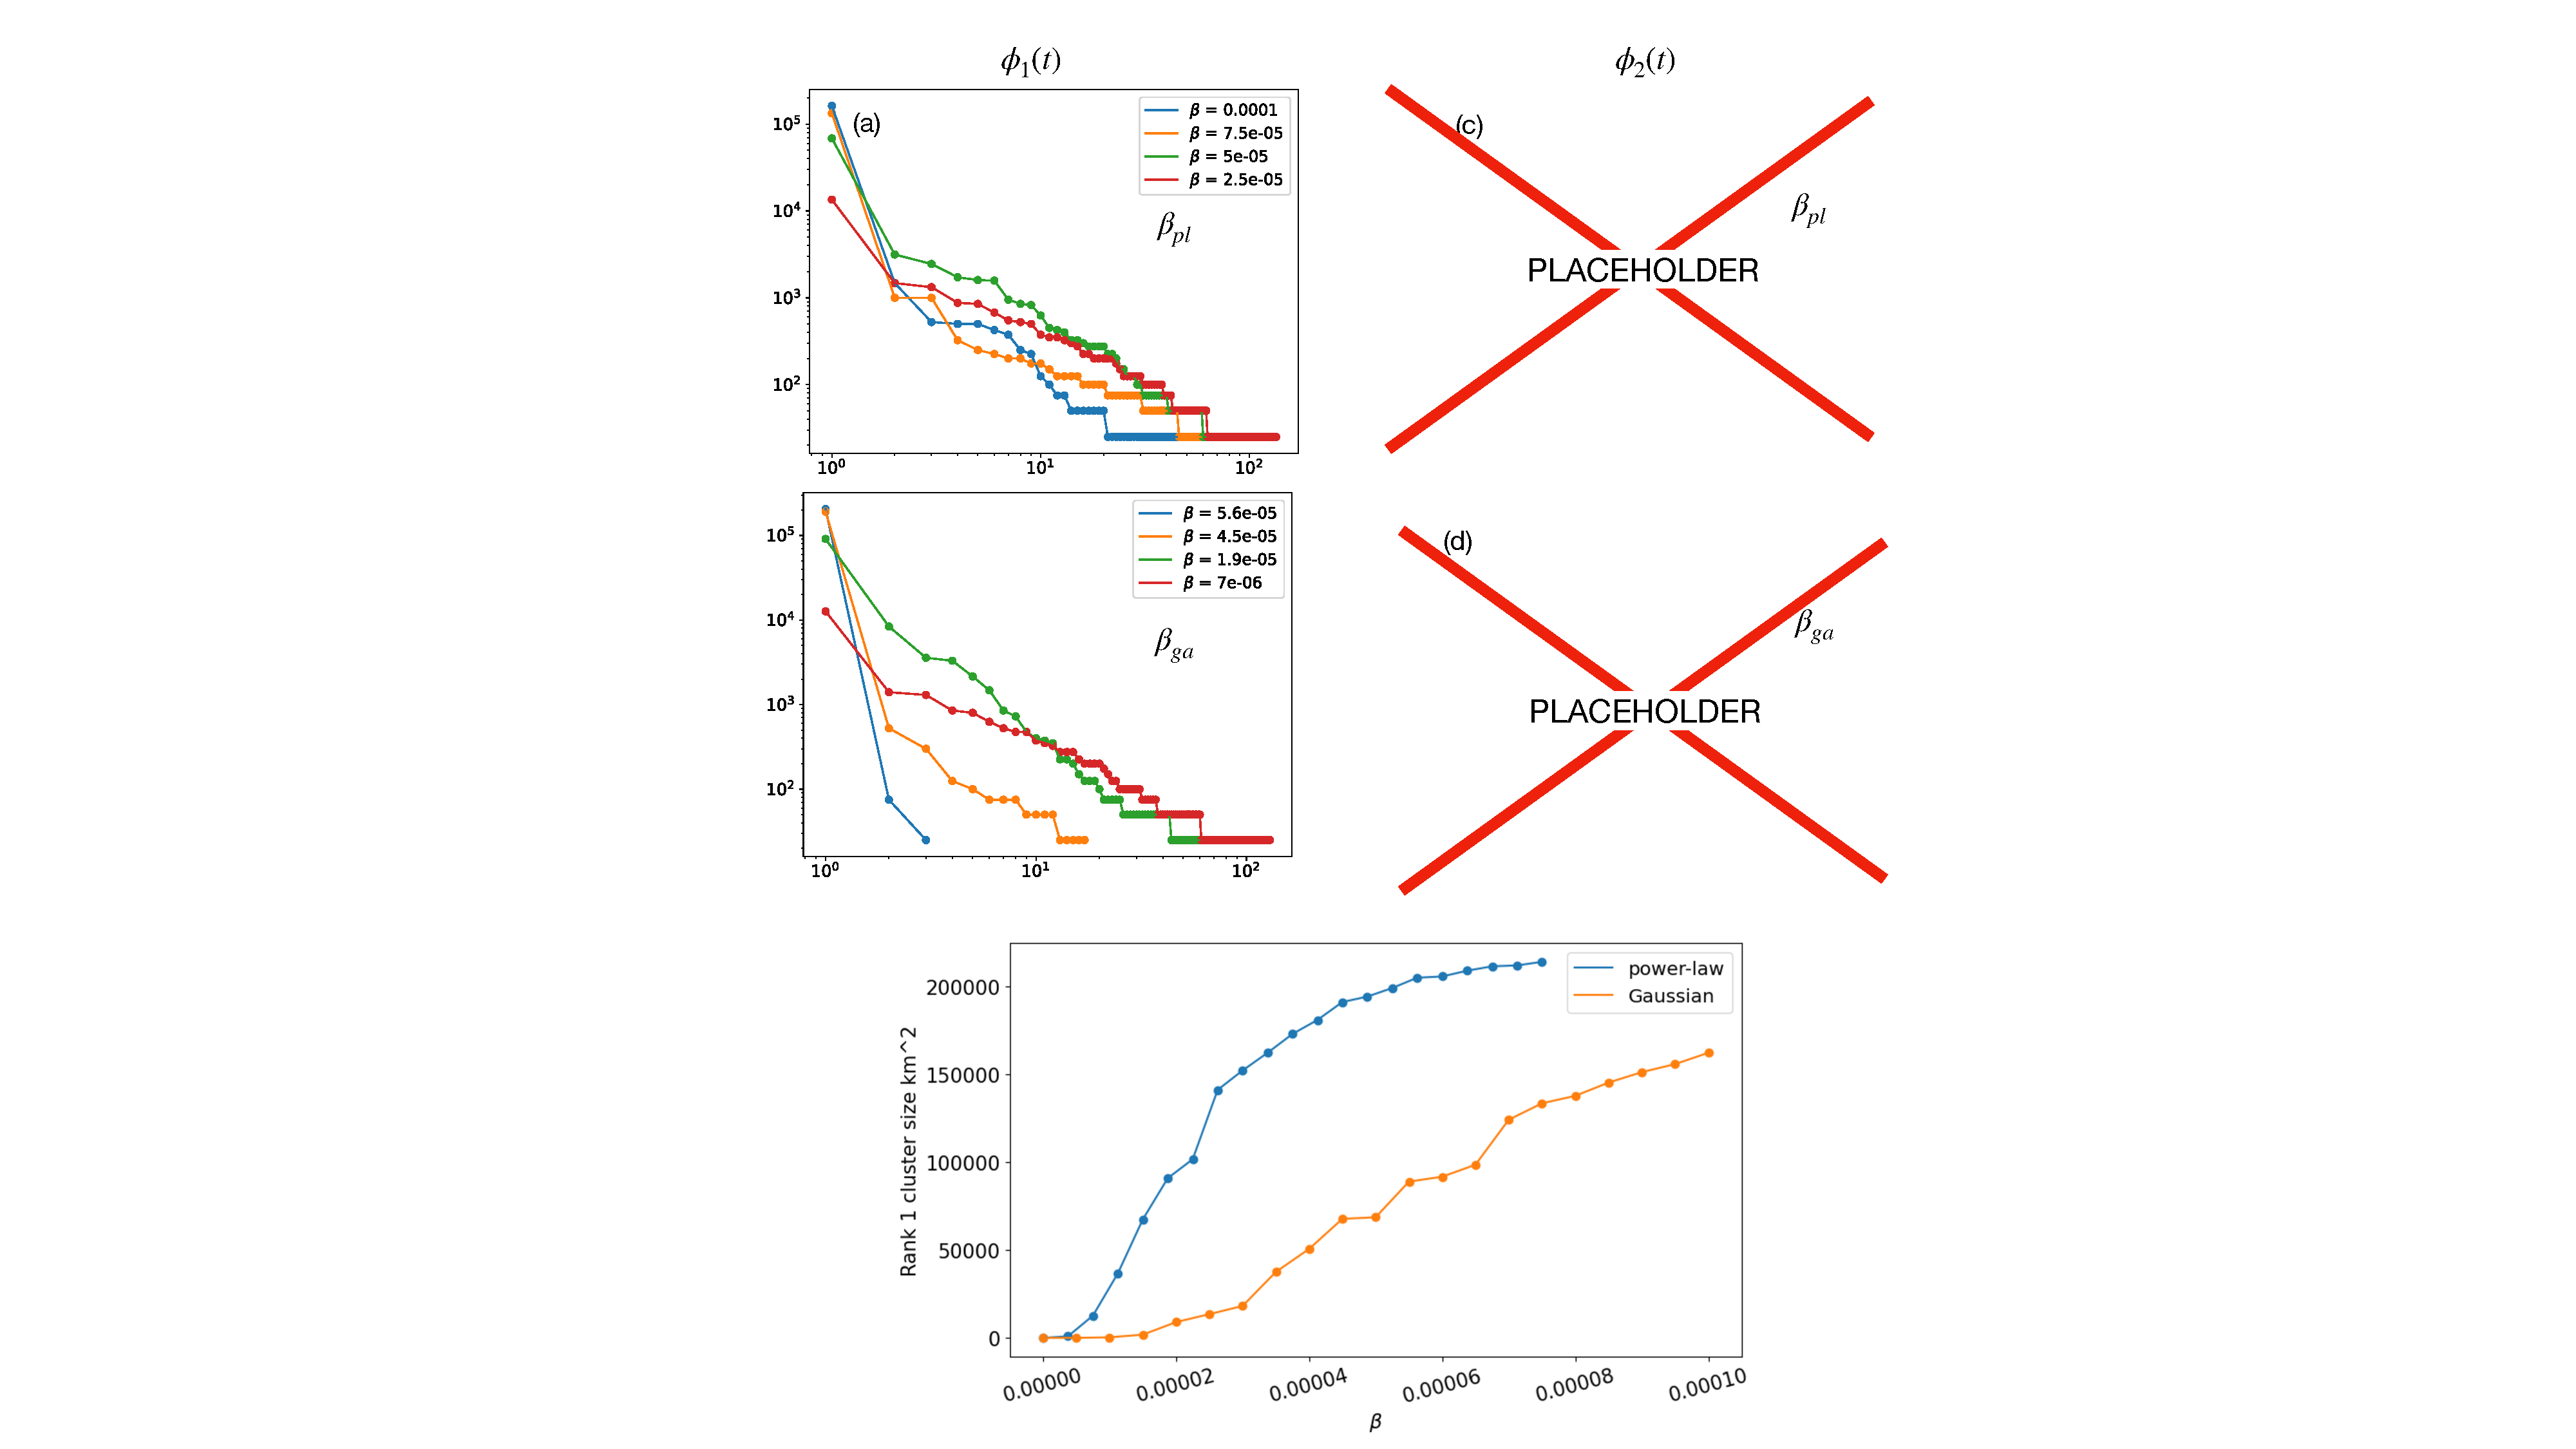
\includegraphics[scale=0.55]{chapter6/figures/fig6-cluster-size-distribution.pdf}. % replace figures with correct sporulation functions and Gaussian.
    \caption{I am a place holder.}
    \label{fig:my_label}
\end{figure}


\blindtext % introduce the largest cluster figure, and large jumps

\blindtext. % explain why different scaling of beta ?




\section{Chapter summary}

% Where we consider spatial structure and others have not
% - In this chapter, we focused on disrupting local-level dispersal by implementing control at landscape-level.
% -  In this chapter we undertook the ambitious task of scaling up a small-scale model, to large spatial distances covering GB, and developed a new approach to controlling the spread of disease.
% - introduce the regime of pathogen spread we are interested in, we are not modelling continental long-range spread via upper atmosphere, nor are we interested in long-range human trade networks. We are interested in dispersal at the local level whereby passive means of wind, soil and or insects/animals. 

These results are focused toward help policy makers implement informed decisions, about \textit{where} to control the spread of disease, based on spatial arguments, when budgets are low\textemdash as noted by \cite{time-varying-infectivity}. Our approach of spatially scaling small-scale epidemiological principles was conducted through computational, opposed to analytical, means. 

The article published by \cite{time-varying-infectivity} indicates the possibility of \textit{preferentially} controlling an area based on the final-sized epidemic. It goes without saying that areas of land that have the largest final sized epidemic are likely the most density populated. However, we outline the possibility it might be more beneficial to preferentially control an area based on its spatial location and how it couples to to neighbouring areas.

% The scaling up of our model
The scaling up of our model resembles a metapopulation model, now commonplace when modelling plant-based epidemics, but crucially our large-scale model is not dynamic. A dynamic large-scale model is indeed useful for the prediction of time-scales and the movement of disease-fronts movement; however, we suggest they might be at best less useful for optimised large-scale control, and at worse, nicely complemented by the approach we develop.

If early data through a particular region, with known data, was collected, it would be a relatively short step to fit the dispersal model and scale up the model over large distances given the seemingly simple relation to host density $\rho$.
% At the small scale we have a uniform population. However for larger scales we have considerable spatial heterogeneity.
% spatial-scale and control, over a multi-seasonal pathosystem, have been investigated for sugar beet in the UK, see \cite{doi:10.1146/annurev.phyto.45.062806.094357} for a review.

% On the SEIR model

The cyclic nature of the $SEIR$-type model constructed in this article can also find resemblance in the, well established body of literature, of crop-based epidemics. It is common-place for a field of crops to become infested, then at the end of the growing season be totally eradicated by virtue of harvesting % \cite{time-varying-infectivity} has 
% we contend the SnIEmR model, considered over one sporulation peak, is a simplistic implementation of the SEIR-based model needed to compute an invasion threshold that represent the infection dynamics ash dieback. 
% The SEIR-based model is made more flexible, and can be readily extended or adapted to incorporate more biological realism, by virtue of splitting the E and I into multiple compartments\textemdash this is frequently done in human and animal-based models \citations..

%- Although the main result of our work was conduced over one sporulation peak, or life-cycle of ash dieback, splitting the model into various compartments was a useful and necessary step towards developing accurate large-tree species. reference  \cite{https://doi.org/10.1111/ppa.12894} alludes to multiple exposed periods being useful

%- A quantity of interest that appears frequently in the literature is the initial growth rate $r$, that is the density-independent growth at the start of any epidemic.
% See \cite{ferrandino2012time} for a review on the time-scales and sporulation of plant-based diseases.

% Fitting data to the early phases of an epidemic has been shown to give large differences in the final-size epidemic, or severity \cite{time-varying-infectivity}. However, we are only interested in a pathogens ability to invade and this can be closely approximated by measuring R0 over the fist observation (\see appendix)

% The variability between the particular life-cycle history followed by hosts is thought to be an important factor to consider\cite{ferrandino2012time}, and we intentionally neglected this for the purpose of simplicity...

% \footnote{A review on the landscape epidemiology of ADB \cite{doi:10.1111/1365-2745.13383} concluded that the effect of host abundance in the neighborhood of ADB decayed with distance, according to an exponential distribution with scale parameter $200\mathrm{m}$. That is, the severity of ADB symptoms depended on the surrounding abundance of ash.} 
% 

% Accurately modelling time-varying infectivity is difficult \cite{13-challenges}, and as such, we opted for parsimony.

% Main assumptions in the method: 
% 1) Assumptions about dispersal
Dispersal over small spatial-scale is thought to predominately occur passively through wind, however other means of dispersal exist such as soil and or insects. There are many pathways a pathogen can use to spread through a landscape, including long-range dispersal, mediated through either human-trade networks %
\cite{hulme2009trade, banks2015role, chapman2017global} or dispersal in the upper atmosphere \cite{westbrook1999atmospheric, isard2005principles}.  

% \textcolor{red}{The last insightful observation from Figure \ref{fig:max_dist_vs_R0} relates to the averaging spreading velocity of ADB...}
% We assumed some regions can sustain an epidemic and some cannot, we assume that $R_0>1$ is the threshold separating these regimes.

% 2) Assumptions about R0
To our knowledge, $R_0$ has not been estimated for Ash dieback, or indeed for any large deciduous tree species, unlike for some crop-based pathogens \cite{segarra2001epidemic}. The lack of $R_0$-estimates made it hard to scrutinize which $\beta$-valued $R_0$-map would be likely to reflect reality. This gap in the body of literature is hardly surprising given the complexity of measuring time-varying infectivity rates \cite{13-challenges}. Thus, as it stands, our results hint-towards the utility of landscape-level control but come short of definitive proof.

% Looking at \cite{R0-perc-ref}, it makes me think our notion of $R_0$ is pretty simplistic. We only measure the local-level $R_0$. We do not consider $R_0$ from patch to patch. What scale we measure $R_0$ has a huge impact on what the result is. Could we rank land-patches not only on there local $R_0$ level, but also on the impact they have on there immediate neighbours ? This would, in theory be an improvement to the clustering algorithm.

% A map of $R_0$ values is useful to policy makers and plant modelers alike.

% Improvements to the model:
% 1) The algorithm
% The algorithm to target not only the critically connecting patches, but also find fragmenting lines which minimise risk at the landscape-level ? Incorporating the local impact a particular patch may have on its neighbours.
% 2) Multi-year R0 analysis
% However, we .... xyz cover all basis of using a one-season approximation. <- this leads to a risk-based argument in which we could capture a 2nd-order R0 which does, xyz. We mainly interested in a pathogens ability to invade. 

% Analysis was aired towards simplicity, a more expansive study with e.g. more sophisticated sporulation functions could be the subject of future work.

% The most important message of our work was...
% The spatial and temporal scale of the control-strategy should match intrinsic spatial and temporal scale of the invasion. <- Hence R0 measured over one season. 


% our modelling approach and results are in their infancy,  

% Last remarks and future modelling work:
To our knowledge, there is a surprising lack of spatio-temporal ADB models exist in the literature, probably because of the significant challenges involved in containment. Although our findings are far from complete, it suggests the spread of ash dieback, between spatial locations, could be reduced by preferentially targeting sites to minimise epidemiological connectivity. Not surprisingly, more work will need to be done to ascertain the degree to which this strategy could impede the spread. 

% Crucially, future work will involve integrating LDD mechanisms into the model in order to understand the relative importance long vs local distance dispersal. We may speculate about the relative importance looking at figure x, whereby the maximum distance spread in season due to local-scale spread is xm/year, in stark contrast from the observed spread of 40-60km/yr.

% We cannot overstate the importance of LDD, and it is hard to say the degree to which targeting the local dispersal mechanism alone will inhibit the spread. We will revisit this question in future work, however, we contend that preferentially targeting diseased trees based on spatial location.....could help control epidemics with greater efficacy. 

% We may speculate how our result could aid the effort of choosing where to re-plant ash stands genetically engineered to be less susceptible; if re-planting efforts were undertaken in certain location.... <- speculative

% We may speculate about how persistent ash dieback would be, even if a large-scale control effort was undertaken

% There is evidence to suggest regional variation in mortality due to ash dieback \cite{stocks2017first}, this could be incorporated into the model...

% Our results support the call for more research to be undertaken into multi-scale dispersal, 

% Recently, it has been suggested that the dispersal-kernel of wind-borne pathogens might follow a scaling law \cite{https://doi.org/10.1111/jbi.13642}. The significance of such a finding would allow us to analyse the $R_0$-maps over much more flexible spatial scales. % Explain.

% This sentence is wrong, the cited paper makes an argument for the spatially-scaling up of dispersal kernels, which happens to still be useful paper to cite, re-phrase and re-frame accordingly.

% see \cite{ash-dieback-costs}, and the references therein (methodology excel spread sheet S1), for mortality references the latest findings suggest a mean mortality rate of 95%.



